% ==============================================================================
% FICHIER PRINCIPAL : main.tex
% Projet de Fin d'Études : SafeCity-Connect
% Auteurs : Dhia Fersi & Mohamed Iyed Amiri (ISET Bizerte)
% Organisme d'accueil : HRMAPS
% ==============================================================================

\documentclass[12pt,a4paper,oneside]{report}

\usepackage[table]{xcolor} % Pour colorer les cellules des tableaux de la page de garde


% ------------------------------------------------------------------------------
% 1. Encodage et Langue
% ------------------------------------------------------------------------------
\usepackage[utf8]{inputenc}
\usepackage[T1]{fontenc}
\usepackage[french]{babel}

% ------------------------------------------------------------------------------
% 2. Police et Style de Texte (Times New Roman)
% ------------------------------------------------------------------------------
\usepackage{mathptmx} % Police Times New Roman de haute qualité
\usepackage{setspace}
\onehalfspacing % Interligne 1.5
\usepackage{microtype} % Pour optimiser la justification et éviter les grands espaces entre les mots


% ------------------------------------------------------------------------------
% 3. Marges (2.5 haut/bas, 3 gauche, 2 droite)
% ------------------------------------------------------------------------------
\usepackage[top=2.5cm, bottom=2.5cm, left=3cm, right=2cm]{geometry}

% ------------------------------------------------------------------------------
% 4. Espacement des Paragraphes
% ------------------------------------------------------------------------------
\setlength{\parskip}{6pt} % Espacement de 6pt entre les paragraphes
\setlength{\parindent}{0.75cm} % Retrait de paragraphe standard
\usepackage{indentfirst} % Indenter le premier paragraphe après un titre

% ------------------------------------------------------------------------------
% 5. Titres et Espacements (Même niveau vertical, tailles distinctes)
% ------------------------------------------------------------------------------
\usepackage{titlesec}
\usepackage{amssymb} % Pour les symboles de puces (carré)

% Format des chapitres
\titleformat{\chapter}[block]
  {\normalfont\LARGE\bfseries\raggedright}
  {\chaptertitlename\ \thechapter\quad }
  {0pt}
  {\LARGE}
\titlespacing*{\chapter}{0pt}{12pt}{6pt}

% Format des sections (1.)
\titleformat{\section}[block]
  {\normalfont\Large\bfseries\raggedright}
  {\thesection.\quad }
  {0pt}
  {\Large}
\titlespacing*{\section}{0pt}{6pt}{6pt}

% Format des sous-sections (1.1.)
\titleformat{\subsection}[block]
  {\normalfont\large\bfseries\raggedright}
  {\thesubsection.\quad }
  {0pt}
  {\large}
\titlespacing*{\subsection}{0pt}{6pt}{6pt}

% Format des sous-sous-sections (1.1.1.)
\titleformat{\subsubsection}[block]
  {\normalfont\normalsize\bfseries\itshape\raggedright}
  {\thesubsubsection.\quad }
  {0pt}
  {\normalsize\itshape}
\titlespacing*{\subsubsection}{0pt}{6pt}{6pt}

% ------------------------------------------------------------------------------
% 6. Numérotation et Pagination
% ------------------------------------------------------------------------------
% Profondeur de numérotation et de table des matières (jusqu'à 1.1.1.a)
\setcounter{secnumdepth}{4}
\setcounter{tocdepth}{4}

% Redéfinition de la numérotation (Section = 1, Subsection = 1.1, Subsubsection = 1.1.1, Paragraph = 1.1.1.a)
\renewcommand{\thechapter}{\arabic{chapter}}
\renewcommand{\thesection}{\arabic{section}}
\renewcommand{\thesubsection}{\thesection.\arabic{subsection}}
\renewcommand{\thesubsubsection}{\thesubsection.\arabic{subsubsection}}
\renewcommand{\theparagraph}{\thesubsubsection.\alph{paragraph}}

% Format de paragraphe (1.1.1.a) comme un titre de bloc
\titleformat{\paragraph}[block]
  {\normalfont\normalsize\bfseries\raggedright}
  {\theparagraph.\quad }
  {0pt}
  {\normalsize}
\titlespacing*{\paragraph}{0pt}{6pt}{6pt}

% ------------------------------------------------------------------------------
% 7. En-têtes et Pieds de Page (fancyhdr)
% ------------------------------------------------------------------------------
\usepackage{fancyhdr}
\pagestyle{fancy}
\fancyhf{} % Nettoyer en-têtes et pieds par défaut

% En-tête
\fancyhead[L]{\nouppercase{\leftmark}} % Titre du chapitre courant
\fancyhead[R]{SafeCity-Connect} % Titre du projet
\renewcommand{\headrulewidth}{0.4pt} % Ligne séparatrice fine

% Pied de page
\fancyfoot[C]{\thepage} % Numéro de page au centre
\renewcommand{\footrulewidth}{0pt} % Pas de ligne en bas

% Redéfinir le style "plain" pour les débuts de chapitres
\fancypagestyle{plain}{
  \fancyhf{}
  \fancyfoot[C]{\thepage}
  \renewcommand{\headrulewidth}{0pt}
}

% ------------------------------------------------------------------------------
% 8. Puces et Listes Uniformes (enumitem)
% ------------------------------------------------------------------------------
\usepackage{enumitem}
% Définition des symboles de puces par niveau (point, cercle, tiret, carré)
\setlist[itemize,1]{label=$\bullet$, leftmargin=1.5cm, topsep=4pt, itemsep=2pt, parsep=0pt}
\setlist[itemize,2]{label=$\circ$, leftmargin=1.2cm, topsep=3pt, itemsep=2pt, parsep=0pt}
\setlist[itemize,3]{label={--}, leftmargin=1.0cm, topsep=3pt, itemsep=2pt, parsep=0pt}
\setlist[itemize,4]{label=$\blacksquare$, leftmargin=0.8cm, topsep=3pt, itemsep=2pt, parsep=0pt}

% Pour les listes numérotées
\setlist[enumerate,1]{label=\arabic*., leftmargin=1.5cm}
\setlist[enumerate,2]{label=\alph*., leftmargin=1.2cm}

% ------------------------------------------------------------------------------
% 9. Gestion des Images, Tableaux et Liens
% ------------------------------------------------------------------------------
\usepackage{graphicx}
\usepackage{booktabs} % Pour des tableaux professionnels
\usepackage{tabularx} % Tableaux à largeur ajustable
\usepackage{hyperref} % Liens cliquables
\hypersetup{
    colorlinks=true,
    linkcolor=black, % Liens noirs pour l'impression du rapport
    filecolor=black,
    urlcolor=blue,
    citecolor=black
}
\usepackage{float} % Pour forcer le positionnement des images (H)

% Dossier contenant les images et logos
\graphicspath{{./}{./rapport/}}

% ------------------------------------------------------------------------------
% DOCUMENT PRINCIPAL
% ------------------------------------------------------------------------------
\begin{document}

% --- PARTIE INITIALE (Pagination en chiffres romains) ---
\pagenumbering{roman}

% Page de garde
% ==============================================================================
% FICHIER : page_de_garde.tex
% Description : Page de garde officielle de l'ISET Bizerte
% Auteurs : Dhia Fersi & Mohamed Iyed Amiri (ISET Bizerte)
% Organisme d'accueil : HRMAPS
% ==============================================================================

\thispagestyle{empty} % Pas d'en-tête ni de pied de page pour la page de garde

% --- EN-TÊTE OFFICIEL DE LA PAGE DE GARDE (Trois colonnes : ISET, Textes, HRMAPS) ---
\noindent
\begin{minipage}[c]{0.18\textwidth}
    \centering
    
\includegraphics[width=\linewidth]{logo iset.jpg}
\end{minipage}
\hfill
\begin{minipage}[c]{0.60\textwidth}
    \centering
    \footnotesize
    Ministère de l'Enseignement Supérieur et de la Recherche Scientifique \\
    Direction Générale des Études Technologiques \\
    \textbf{Institut Supérieur des Études Technologiques de Bizerte} \\
    Département Technologies de l'Informatique
\end{minipage}
\hfill
\begin{minipage}[c]{0.18\textwidth}
    \centering
    
\includegraphics[width=\linewidth]{hrmaps logo.jpg}
\end{minipage}

\vspace{0.2cm}
\hrule height 0.8pt
\vspace{0.2cm}

% --- TABLEAU DES CODES DÉPARTEMENT / ANNÉE / RÉFÉRENCE ---
\noindent
\begin{tabular}{|l|p{2.5cm}|}
    \hline
    \textbf{DEP.} & \textbf{TI} \\ \hline
    \textbf{AN.} & \textbf{2026} \\ \hline
    \textbf{REF.} & \\ \hline
\end{tabular}

% --- TITRES ACADÉMIQUES ---
\begin{center}
    \vspace{0.2cm}
    {\large Rapport de}\\[0.1cm]
    {\Large\bfseries PROJET DE FIN D'ÉTUDES}\\[0.2cm]
    {\large En vue de l'obtention de :}\\[0.15cm]
    {\Large\bfseries Licence en Technologies de l'Informatique}\\[0.1cm]
    {\large\bfseries Parcours : Développement des Systèmes d'Information (DSI)}\\
\end{center}

% --- CADRE DE TITRE DE PROJET ---
\vspace{0.3cm}
\noindent
\centering
\framebox[\linewidth]{
    \parbox{0.94\linewidth}{
        \centering
        \vspace{0.3cm}
        {\Huge\bfseries SafeCity-Connect} \\
        \vspace{0.2cm}
        {\large Plateforme Citoyenne Connectée de Signalement \\ et d'Analyse des Incidents Urbains assistée par IA}
        \vspace{0.3cm}
    }
}

% --- BLOC DES AUTEURS ---
\begin{center}
    \vspace{0.3cm}
    {\large Élaboré par :}\\[0.1cm]
    {\large\bfseries M. Dhia FERSI}\\[0.02cm]
    {\small\bfseries \&}\\[0.02cm]
    {\large\bfseries M. Mohamed Iyed AMIRI}\\
\end{center}

\vspace{0.3cm}

% --- BAS DE PAGE (Encadrants et Entreprise) ---
\noindent
\begin{minipage}[t]{\textwidth}
    \raggedright
    {\large\bfseries Encadré par :}\\[0.1cm]
    \textbf{Mme. Nadia Hachani (ISET Bizerte)} \\
    \textbf{M. Rami Bouafif (HRMAPS)} \\
    
    \vspace{0.3cm}
    {\large\bfseries Effectué à :}\\[0.1cm]
    \textbf{Entreprise : HRMAPS}
    \begin{itemize}[leftmargin=0.4cm, label=\textbullet, noitemsep, topsep=1pt]
        \item \textbf{Adresse :} Immeuble Promed, Bloc B, 7ème étage, Centre Urbain Nord, Tunis 1082
        \item \textbf{Tel :} +216 71 883 780
        \item \textbf{Mail :} contact@hrmaps.fr
    \end{itemize}
\end{minipage}

\vfill

% --- ANNÉE UNIVERSITAIRE ---
\begin{center}
    \rule{0.3\linewidth}{0.6pt}\\[0.1cm]
    {\large\bfseries Année universitaire : 2025/2026}
\end{center}

\newpage

% Dédicaces & Remerciements
% ==============================================================================
% FICHIER : dedicaces_remerciements.tex
% Description : Dédicaces et Remerciements
% Auteurs : Dhia Fersi & Mohamed Iyed Amiri (ISET Bizerte)
% Organisme d'accueil : HRMAPS
% ==============================================================================

% ------------------------------------------------------------------------------
% DÉDICACES (Dhia Fersi)
% ------------------------------------------------------------------------------
\thispagestyle{plain}
\chapter*{Dédicaces}
\addcontentsline{toc}{chapter}{Dédicaces}

\begin{flushright}
    \itshape
    Je dédie ce travail : \\
    
    À mes chers parents, pour leur amour inconditionnel, \\
    leur soutien indéfectible et les sacrifices consentis \\
    pour mon éducation et ma réussite. \\
    Aucun mot ne saurait exprimer ma gratitude. \\
    
    À mes enseignants de l'ISET Bizerte, pour leur dévouement \\
    et la qualité de la formation qu'ils nous ont prodiguée. \\
    
    À mon cher binôme, Mohamed Iyed Amiri, pour son esprit \\
    de collaboration, son sérieux et son amitié. \\
    
    À tous mes amis et à tous ceux qui ont contribué, \\
    de près ou de loin, à la réalisation de ce travail. \\
    
    \vspace{1.5cm}
    \textbf{Dhia Fersi}
\end{flushright}

\newpage

% ------------------------------------------------------------------------------
% DÉDICACES (Mohamed Iyed Amiri)
% ------------------------------------------------------------------------------
\thispagestyle{plain}
\chapter*{Dédicaces}

\begin{flushright}
    \itshape
    Je dédie ce modeste travail : \\
    
    À ma famille, qui a toujours cru en moi, m'a soutenu \\
    durant mes moments de doute et m'a encouragé \\
    tout au long de mes études. \\
    
    À mes formateurs et professeurs, pour leur encadrement \\
    et le partage généreux de leur savoir. \\
    
    À mon binôme, Dhia Fersi, pour cette belle aventure \\
    de projet de fin d'études et sa collaboration constructive. \\
    
    À tous ceux que j'aime et qui me sont chers. \\
    
    \vspace{1.5cm}
    \textbf{Mohamed Iyed Amiri}
\end{flushright}

\newpage

% ------------------------------------------------------------------------------
% REMERCIEMENTS
% ------------------------------------------------------------------------------
\thispagestyle{plain}
\chapter*{Remerciements}
\addcontentsline{toc}{chapter}{Remerciements}

\noindent
Au terme de ce Projet de Fin d'Études, c'est un agréable devoir de témoigner notre reconnaissance et d'exprimer nos vifs remerciements à toutes les personnes qui nous ont aidés dans la réalisation de ce travail.

Nous tenons tout d'abord à exprimer notre profonde gratitude à notre organisme d'accueil, \textbf{HRMAPS}, de nous avoir accueillis et offert l'opportunité de travailler sur un projet aussi passionnant et formateur que \textit{SafeCity-Connect}.

Nos remerciements les plus sincères s'adressent également à notre encadrant professionnel au sein de HRMAPS, \textbf{M. Rami Bouafif}, pour son accueil chaleureux, sa disponibilité, ses conseils judicieux et son accompagnement précieux tout au long de ce stage.

Nous exprimons notre vive reconnaissance à notre encadrante universitaire à l'\textbf{ISET Bizerte}, \textbf{Mme. Nadia Hachani}, pour sa direction rigoureuse, ses suggestions constructives et ses encouragements réguliers qui ont grandement facilité la rédaction de ce rapport.

Enfin, nous remercions les membres du jury d'avoir accepté d'évaluer notre travail et de nous faire l'honneur de présider notre soutenance.

\newpage

% Table des matières, des figures et des tableaux
\tableofcontents
\newpage
\listoffigures
\newpage
\listoftables
\newpage

% --- CORPS DU TEXTE (Pagination en chiffres arabes dès l'Intro Générale) ---
\pagenumbering{arabic}
\setcounter{page}{1} % Force le commencement de la page 1

% Introduction générale
% ==============================================================================
% FICHIER : introduction_generale.tex
% Description : Introduction Générale du rapport SafeCity-Connect
% Auteurs : Dhia Fersi & Mohamed Iyed Amiri (ISET Bizerte)
% Organisme d'accueil : HRMAPS
% ==============================================================================

\chapter*{Introduction Générale}
\addcontentsline{toc}{chapter}{Introduction Générale}

La progression rapide du paysage technologique contemporain a propulsé la transformation numérique au rang d'enjeu stratégique majeur pour l'ensemble des organisations, qu'elles relèvent du secteur public ou privé. Adopter des solutions informatiques performantes constitue aujourd'hui un levier indispensable pour se défaire des processus archaïques, accélérer le traitement de l'information et offrir aux citoyens des prestations fiables, agiles et en adéquation avec leurs attentes croissantes.

À cet égard, la gouvernance des espaces urbains et la gestion du domaine public appellent la mise en place de dispositifs technologiques novateurs favorisant l'implication collective. Les autorités municipales se trouvent en effet confrontées, au quotidien, à un éventail de dysfonctionnements sur la voie publique~-- nids-de-poule, ruptures de canalisations, pannes du réseau d'éclairage ou accumulations illicites de déchets~-- qui altèrent significativement la qualité de vie des résidents tout en générant des charges d'entretien considérables. Le paradigme des villes intelligentes (Smart Cities) offre des solutions tangibles à ces défis en promouvant une approche participative de la gestion urbaine, où le citoyen devient un acteur central du signalement et où les responsables territoriaux disposent d'outils analytiques robustes pour piloter les interventions.

C'est précisément dans ce contexte que s'inscrit notre projet de fin d'études, réalisé au sein de l'entreprise \textbf{HRMAPS}. L'objectif principal a porté sur la conception et l'élaboration de \textbf{SafeCity-Connect} : une plateforme de signalement géolocalisé et de suivi des incidents urbains. Elle combine un \textbf{backend Spring Boot} monolithique, un portail \textbf{Angular~18} (carte publique sans connexion, espaces citoyen, administrateur et services techniques), une application \textbf{Flutter}, l'authentification \textbf{Keycloak}, une base \textbf{PostgreSQL/PostGIS} et un service \textbf{FastAPI/YOLOv8} pour la classification automatique des photos.

Ce rapport retrace de façon détaillée l'ensemble des étapes de réalisation et de maturation de ce projet. Sa structure se décline selon l'articulation suivante :

Le premier chapitre, \textbf{« Présentation du cadre du projet »}, expose l'organisme d'accueil \textbf{HRMAPS} ainsi que son fonctionnement interne. Il dresse un état des lieux critique des pratiques existantes afin de mettre en lumière leurs limites et de légitimer la solution envisagée. Ce chapitre précise en outre les orientations méthodologiques retenues (associant Scrum et UML), les ressources matérielles mobilisées et le schéma d'architecture n-tiers adopté.

Le deuxième chapitre, intitulé \textbf{« Analyse et spécification des besoins »}, procède au recensement des acteurs impliqués, à la formalisation des exigences fonctionnelles et non fonctionnelles du système, et à l'ordonnancement des travaux au travers du carnet de produit (Product Backlog).

Le troisième chapitre, dédié à la \textbf{« Release 1 : Gestion d'accès, profils et sécurité »}, décrit l'édification du socle sécuritaire centralisé fondé sur \textbf{Keycloak}, l'administration des profils utilisateurs, et les premières briques d'implémentation (Sprint 0 et livrables fondamentaux).

Le quatrième chapitre, portant sur la \textbf{« Release 2 : Gestion avancée, rapports et intelligence artificielle »}, traite de l'affectation aux services techniques, des preuves de réparation, des tableaux de bord et heatmap, de la classification YOLOv8, des alertes administrateur dédiées aux nouveaux reports à vérifier, du support par tickets et de la gamification (+10 points à la validation).

Pour clore ce mémoire, une conclusion générale synthétise les résultats obtenus au regard des objectifs fixés et esquisse les axes d'amélioration et d'extension envisageables pour le projet.

\newpage

% Chapitre 1 : Étude préalable
% ==============================================================================
% FICHIER : chapitre1.tex
% Description : Chapitre 1 : Étude préalable
% Auteurs : Dhia Fersi & Mohamed Iyed Amiri (ISET Bizerte)
% Organisme d'accueil : HRMAPS
% ==============================================================================

\chapter{Étude préalable}

\section*{Introduction}
\addcontentsline{toc}{section}{Introduction}
Ce premier chapitre est consacré à l'étude préalable de notre projet de fin d'études. Cette étape permet d'analyser le contexte général du projet, de comprendre le fonctionnement de notre organisme d'accueil, d'évaluer l'existant avec ses forces et ses limites, et de proposer une solution pertinente et adaptée. Il pose les fondations méthodologiques et fonctionnelles nécessaires pour le bon déroulement du projet.

% ------------------------------------------------------------------------------
% 1. PRÉSENTATION DE L'ORGANISME D'ACCUEIL
% ------------------------------------------------------------------------------
\section{Présentation de l'organisme d'accueil}

\subsection{Présentation générale}
L'organisme d'accueil choisi pour la réalisation de ce Projet de Fin d'Études est \textbf{HRMAPS}.

Fondée initialement à Lyon (France) en 2014, HRMAPS s'est positionnée comme un éditeur de logiciels innovant, spécialisé dans le Talent Management (gestion des talents). En 2018, la société franchit un cap stratégique majeur en intégrant le \textbf{Groupe OCTIME}, l'un des leaders européens de la gestion des temps, de la planification et des solutions RH en mode SaaS (Cloud).

Pour piloter ses activités, assurer le déploiement technique et accompagner la transformation digitale des entreprises en Tunisie et sur toute la région de l'Afrique du Nord, la solution s'appuie sur une structure d'intégration et d'expertise locale. Présente en Tunisie depuis 2008, cette structure apporte l'expertise technique et la proximité nécessaires pour adapter l'outil international aux spécificités juridiques, fiscales et organisationnelles du marché tunisien.

Le tableau \ref{tab:identite_entreprise} résume les informations administratives, géographiques et juridiques majeures de notre organisme d'accueil :

\begin{table}[H]
    \centering
    \caption{Fiche d'identité de HRMAPS Tunisie}
    \label{tab:identite_entreprise}
    \vspace{0.3cm}
    \begin{tabularx}{\textwidth}{l X}
        \toprule
        \textbf{Libellé} & \textbf{Description} \\
        \midrule
        \textbf{Raison Sociale} & HRMAPS (Membre du Groupe OCTIME) \\
        \textbf{Secteur d'Activité} & Technologies de l'Information (IT) \& Édition de Logiciels \\
        \textbf{Domaine de Spécialisation} & Solutions de Gestion, SIRH et Management des Talents \\
        \textbf{Modèle Économique} & Solutions Cloud / SaaS (Software as a Service) \\
        \textbf{Adresse du Siège Local} & Immeuble Promed, Bloc B, 7ème étage, Centre Urbain Nord, Tunis 1082, Tunisie \\
        \textbf{Téléphone} & +216 71 883 780 \\
        \textbf{Sites Web Officiels} & \href{https://www.hrmaps.fr}{www.hrmaps.fr} / \href{https://www.octime.com}{www.octime.com} \\
        \textbf{Principaux Clients en Tunisie} & Monoprix, Magasin Général, Géant, ASSAD, OLEA, Boudjebel, etc. \\
        \bottomrule
    \end{tabularx}
\end{table}

\subsection{Services}
L'activité majeure de l'organisme d'accueil gravite autour du déploiement de son SIRH (Système d'Information des Ressources Humaines). La plateforme HRMAPS est une solution modulaire qui automatise et digitalise l'intégralité des processus RH à travers trois grands axes :

\begin{itemize}
    \item \textbf{Le Core RH \& l'Administration} : Centralisation du dossier numérique du collaborateur, portail Self-Service pour la gestion des demandes de congés, des absences et des notes de frais, circuits de validation automatisés (Workflows).
    \item \textbf{La Gestion des Talents} : Digitalisation du recrutement (Suivi des candidats / ATS), processus d'intégration (Onboarding), grilles d'évaluations de performance, cartographie des compétences et plans de formation.
    \item \textbf{Le Pilotage Décisionnel} : Génération automatique de tableaux de bord RH, édition du bilan social et interfaçage natif avec les solutions de paie tierces du marché.
\end{itemize}

\begin{figure}[H]
    \centering
    \framebox[\textwidth]{\vbox to 5cm{\vfill\hbox to \textwidth{\hss\textbf{[Figure : Organigramme structurel de HRMAPS]}\hss}\vfill}}
    \caption{Organigramme structurel de HRMAPS}
    \label{fig:organigramme_hrmaps}
\end{figure}

% ------------------------------------------------------------------------------
% 2. PRÉSENTATION DU PROJET
% ------------------------------------------------------------------------------
\section{Présentation du projet}
Le projet \textbf{SafeCity-Connect} a pour objectif d'apporter une solution technologique innovante en connectant directement les citoyens aux services de maintenance de leur ville, en utilisant le meilleur des technologies du web, du cloud et de l'intelligence artificielle. Il s'agit d'une plateforme citoyenne de signalement géo-localisé des incidents urbains (nids-de-poule, fuites d'eau, pannes d'éclairage public). Le projet simplifie l'interaction citoyenne, automatise la classification des anomalies grâce à l'IA, et fournit aux administrateurs municipaux des outils de pilotage cartographique et statistique.

% ------------------------------------------------------------------------------
% 3. ÉTUDE DE L'EXISTANT
% ------------------------------------------------------------------------------
\section{Étude de l'existant}

\subsection{Analyse de l'existant}
Traditionnellement, la détection et la remontée des anomalies urbaines au sein des communes tunisiennes reposent sur des processus manuels ou semi-manuels :
\begin{itemize}
    \item \textbf{Signalements physiques ou téléphoniques} : Le citoyen doit se déplacer au guichet de la municipalité ou tenter de joindre un standard téléphonique pour déclarer un problème (ex : route endommagée, lampe cassée).
    \item \textbf{Tournées d'inspection planifiées} : Les agents de la voirie effectuent périodiquement des tournées d'inspection pour recenser visuellement les dégâts.
    \item \textbf{Enregistrement papier} : Les requêtes reçues sont transcrites sur des registres physiques ou dans des fichiers Excel isolés, puis transmises manuellement aux équipes de réparation.
\end{itemize}

\subsection{Critique de l'existant}
Ce fonctionnement traditionnel présente de nombreuses failles majeures :
\begin{itemize}
    \item \textbf{Lenteur extrême} : Les délais entre la détection d'une anomalie et son enregistrement effectif par les services techniques peuvent prendre plusieurs semaines.
    \item \textbf{Manque crucial de précision} : Les descriptions verbales ou écrites fournies par les citoyens sont souvent vagues et manquent de coordonnées précises, obligeant les équipes d'intervention à passer du temps à chercher l'incident sur place.
    \item \textbf{Surcharge administrative et erreurs} : La saisie manuelle et le tri des plaintes prennent énormément de temps aux agents municipaux, entraînant parfois la perte ou l'oubli de dossiers.
    \item \textbf{Absence de transparence et de retour d'information} : Les citoyens ne reçoivent aucun suivi de leurs plaintes, ce qui engendre un sentiment de frustration et un désengagement civique total.
\end{itemize}

% ------------------------------------------------------------------------------
% 4. SOLUTION PROPOSÉE
% ------------------------------------------------------------------------------
\section{Solution proposée}
Pour remédier aux lacunes de l'existant, nous proposons le développement de la plateforme \textbf{SafeCity-Connect}, un écosystème logiciel modulaire composé d'une \textbf{application web d'administration (Angular 18)} et d'une \textbf{application mobile multiplateforme (Flutter)} destinée aux citoyens et aux agents de terrain. Ses fonctionnalités phares incluent :
\begin{enumerate}
    \item \textbf{Application Mobile (Flutter)} : Permet aux citoyens de signaler un incident géo-localisé en prenant une photo, de suivre son statut de résolution (fixé ou non) directement sur la carte, de laisser des commentaires, et de donner leur avis après la résolution de l'anomalie (\textit{review fixes}). Elle permet aussi aux agents des départements techniques (dont les comptes sont créés par l'administrateur) de s'authentifier pour visualiser et clore leurs interventions sur site.
    \item \textbf{Catégorisation IA Automatique} : Analyse instantanée de la photo de l'incident par un réseau YOLO pour suggérer automatiquement sa catégorie (nid-de-poule, fuite d'eau, déchets).
    \item \textbf{Système d'Alertes et Notifications par Email} : Envoi automatique d'un e-mail de notification au service d'administration municipale dès qu'un citoyen soumet un nouveau signalement sur la carte de la ville.
    \item \textbf{Portail Web d'Administration (Angular 18)} : Permet de gérer les catégories, de créer les comptes des agents techniques, d'affecter les incidents aux différents départements, de suivre la carte thermique (\textit{Heatmap}) PostGIS et de consulter des indicateurs analytiques.
    \item \textbf{Flux de Clôture et Modération de la Fixation} : L'agent de terrain effectue les travaux et soumet une \textbf{photo preuve de résolution}. L'administrateur étudie cette preuve et peut \textbf{valider} ou \textbf{rejeter} l'intervention en saisissant obligatoirement un \textbf{motif de refus} enregistré dans la timeline de l'incident.
    \item \textbf{Reporting Décisionnel et Exports PDF} : Permet à l'administrateur d'exporter le récapitulatif hebdomadaire des incidents au format Excel/CSV et de générer un rapport PDF individuel complet et officiel pour chaque incident (comprenant les photos avant/après, la timeline interne, les commentaires et les acteurs impliqués).
\end{enumerate}

\section*{Conclusion}
\addcontentsline{toc}{section}{Conclusion}
L'étude préalable réalisée dans ce chapitre nous a permis de justifier pleinement la nécessité de développer la plateforme \textit{SafeCity-Connect}. En analysant l'existant, nous avons mis en lumière les blocages administratifs et opérationnels actuels. La solution proposée offrira une réactivité accrue et modernisera la communication municipale. Le chapitre suivant détaillera la planification du projet ainsi que son architecture globale.

\newpage

% Chapitre 2 : Planification & architecture
% ==============================================================================
% FICHIER : chapitre2.tex
% Description : Chapitre 2 : Planification & architecture
% Auteurs : Dhia Fersi & Mohamed Iyed Amiri (ISET Bizerte)
% Organisme d'accueil : HRMAPS
% ==============================================================================

\chapter{Planification \& architecture}

\section*{Introduction}
\addcontentsline{toc}{section}{Introduction}
La réussite d'un projet informatique complexe repose sur une planification rigoureuse et une architecture logicielle bien pensée. Pour développer \textit{SafeCity-Connect}, nous avons adopté la méthodologie agile \textbf{SCRUM}, réputée pour sa flexibilité et son efficacité de développement. Ce chapitre détaille la spécification des besoins de notre système, présente notre équipe SCRUM, définit le découpage des sprints, expose le Backlog de produit global, et introduit la modélisation fonctionnelle et structurelle à travers les diagrammes UML globaux.

% ------------------------------------------------------------------------------
% 1. SPÉCIFICATION DES BESOINS
% ------------------------------------------------------------------------------
\section{Spécification des besoins}

\subsection{Identification des acteurs du système}
Nous avons identifié quatre acteurs principaux qui interagissent avec la plateforme :
\begin{itemize}
    \item \textbf{Le Citoyen} : Utilise l'application mobile Flutter pour signaler des incidents géolocalisés avec photo, suivre le statut de résolution (fixé ou non) directement sur la carte, laisser des commentaires, et donner son avis sur la réparation finale (\textit{review fixes}).
    \item \textbf{L'Administrateur municipal} : Utilise l'application web Angular pour gérer Keycloak (créer/gérer les comptes des Départements), affecter les interventions, valider/rejeter les preuves de fixation (avec motif obligatoire), analyser la Heatmap, suivre la timeline d'évolution détaillée, recevoir des e-mails d'alertes lors de nouveaux signalements, et exporter les rapports hebdomadaires et fiches d'incidents sous format PDF.
    \item \textbf{Le Département municipal (Agent d'intervention)} : Utilise l'application mobile Flutter pour se connecter via un compte créé par l'admin, consulter ses missions de voirie affectées, effectuer les travaux et soumettre la photo preuve de résolution sur site.
    \item \textbf{Le Système d'IA (YOLO)} : Traite l'image soumise pour classifier automatiquement l'incident.
\end{itemize}

\subsection{Les besoins fonctionnels}
Les besoins fonctionnels décrivent les capacités opérationnelles que doit fournir le système :
\begin{itemize}
    \item \textbf{Gestion d'Identité et Rôles} : Inscription/connexion SSO (Keycloak) pour les citoyens et agents techniques (les comptes Département étant créés manuellement par l'Administrateur).
    \item \textbf{Signalement \& IA (Citoyen)} : Envoi de signalement (photo, localisation Leaflet, classement automatique par YOLO).
    \item \textbf{Commentaires et Revue (Citoyen)} : Ajout de commentaires sur les incidents et validation ou avis après résolution (\textit{review fixes}).
    \item \textbf{Timeline d'Évolution (Admin)} : Fil de vie historique complet (soumission, affectation, réparation, validation/rejet) pour chaque incident, accessible uniquement par l'Administrateur.
    \item \textbf{Affectation \& Modération (Admin)} : Transmission du problème au département idoine ; vérification de la preuve de fixation avec droit d'acceptation ou de rejet motivé (raison obligatoire).
    \item \textbf{Reporting \& Export (Admin)} : Tableau de bord analytique, export hebdomadaire (Excel) et génération de rapports de synthèse au format PDF.
    \item \textbf{Alertes Système} : Envoi instantané d'une notification e-mail à l'Admin lors d'un nouveau signalement citoyen.
    \item \textbf{Opérations terrain (Département)} : Consultation des tâches affectées et transmission de la photo preuve de résolution.
\end{itemize}

\subsection{Les besoins non fonctionnels}
Les besoins non fonctionnels décrivent les caractéristiques de qualité de notre plateforme :
\begin{itemize}
    \item \textbf{Sécurité} : Authentification OAuth2/OIDC gérée centralement par Keycloak pour sécuriser les flux de données.
    \item \textbf{Performance} : Rendu fluide et rapide de la carte thermique et des points, même avec un grand nombre d'incidents (grâce aux index GIST spatiaux sous PostGIS).
    \item \textbf{Ergonomie} : Interface adaptative (\textit{responsive}) respectant les standards du mobile-first pour faciliter l'utilisation sur le terrain.
\end{itemize}

% ------------------------------------------------------------------------------
% 2. STRUCTURE ET DÉCOUPAGE DU PROJET
% ------------------------------------------------------------------------------
\section{Structure et découpage du projet}

\subsection{Identification de l'équipe SCRUM}
L'organisation de notre projet s'articule autour des rôles SCRUM suivants :
\begin{itemize}
    \item \textbf{Product Owners} : Dhia Fersi \& Mohamed Iyed Amiri (en collaboration avec l'encadrant professionnel Rami Bouafif de HRMAPS qui a spécifié les priorités).
    \item \textbf{Scrum Masters} : Dhia Fersi \& Mohamed Iyed Amiri (partage du rôle pour orchestrer le projet).
    \item \textbf{Équipe de Développement} : Dhia Fersi (spécialisé Backend \& PostGIS / IA) \& Mohamed Iyed Amiri (spécialisé Frontend Angular \& Leaflet / Keycloak).
\end{itemize}

\subsection{Découpage des sprints}
Afin de livrer régulièrement des incréments logiciels fonctionnels, nous avons découpé le projet en 5 sprints majeurs (chacun d'une durée de 2 semaines) :
\begin{itemize}
    \item \textbf{Sprint 0} : Mise en place de l'architecture logicielle, infrastructure Docker et technologies de développement.
    \item \textbf{Sprint 1} : Inscription, Authentification unifiée, Gestion de profil et Sécurité via Keycloak.
    \item \textbf{Sprint 2} : Espace Citoyen -- Gestion des Signalements, intégration cartographique Leaflet et analyse photo IA (YOLO).
    \item \textbf{Sprint 3} : Espace Administration -- Tableau de bord, Carte de chaleur spatiale (\textit{Heatmap}) PostGIS et outils de statistiques.
    \item \textbf{Sprint 4} : Espace Gamification -- Historique citoyen, gestion des points d'impact et validation globale.
\end{itemize}

\subsection{Le Backlog du produit}
Le tableau \ref{tab:backlog_produit} résume les récits utilisateurs (\textit{User Stories}) du Backlog Produit :

\begin{table}[H]
    \centering
    \caption{Backlog de Produit SafeCity-Connect}
    \label{tab:backlog_produit}
    \vspace{0.2cm}
    \small
    \begin{tabularx}{\textwidth}{l p{7.5cm} c c c}
        \toprule
        \textbf{ID} & \textbf{User Story (En tant que... Je veux... Afin de...)} & \textbf{Priorité} & \textbf{Complexité} & \textbf{Sprint} \\
        \midrule
        \textbf{US01} & Déployer l'architecture globale conteneurisée. & Haute & 5 & Sprint 0 \\
        \textbf{US02} & M'inscrire, me connecter et gérer mon profil (Citoyen/Dept). & Haute & 8 & Sprint 1 \\
        \textbf{US03} & Créer et gérer les comptes des agents techniques (Admin). & Moyenne & 3 & Sprint 1 \\
        \textbf{US04} & Signaler un incident avec géo-localisation et photo IA. & Haute & 13 & Sprint 2 \\
        \textbf{US05} & Consulter le statut de résolution (fixé/non fixé) sur la carte. & Haute & 3 & Sprint 2 \\
        \textbf{US06} & Affecter des incidents aux départements techniques (Admin). & Haute & 5 & Sprint 3 \\
        \textbf{US07} & Exporter les incidents hebdomadaires et fiches PDF (Admin). & Moyenne & 8 & Sprint 3 \\
        \textbf{US08} & Recevoir des alertes par e-mail lors de signalements. & Moyenne & 5 & Sprint 3 \\
        \textbf{US09} & Uploader une photo preuve de résolution (Département). & Haute & 8 & Sprint 4 \\
        \textbf{US10} & Accepter ou rejeter la fixation avec motif (Admin). & Haute & 8 & Sprint 4 \\
        \textbf{US11} & Échanger des commentaires et évaluer les réparations (Citoyen). & Moyenne & 8 & Sprint 4 \\
        \bottomrule
    \end{tabularx}
\end{table}

\subsection{Planification des releases}
Notre projet prévoit une release intermédiaire après le Sprint 2 (version citoyenne fonctionnelle avec signalement IA) et une release finale de production à la fin du Sprint 4 (version complète avec dashboard d'administration et de gamification).

\subsection{Diagramme de cas d'utilisation global}
Le diagramme de cas d'utilisation global modélise l'ensemble des interactions fonctionnelles autorisées pour chaque acteur (voir Figure \ref{fig:uc_global}).

\begin{figure}[H]
    \centering
    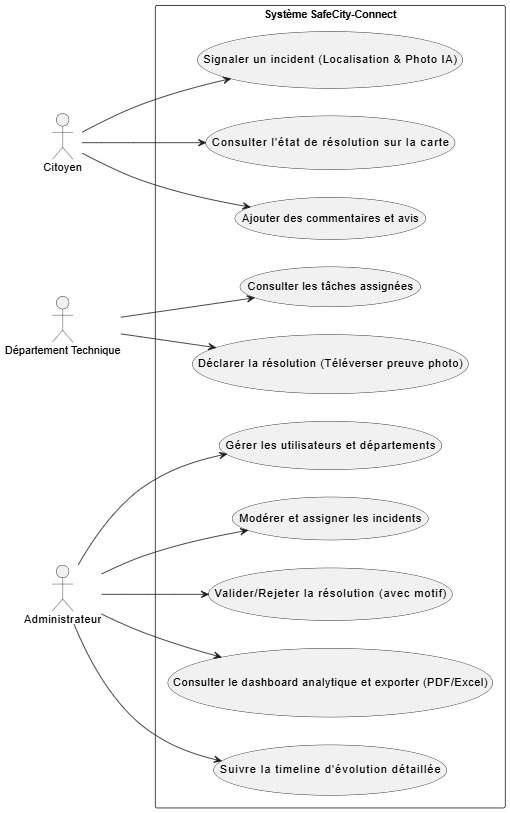
\includegraphics[width=0.9\textwidth]{use_case_global.jpg}
    \caption{Diagramme de cas d'utilisation global de la plateforme}
    \label{fig:uc_global}
\end{figure}

\subsection{Diagramme de classe global (initial)}
Le diagramme de classe global initial présente la structure conceptuelle des données et les relations métiers qui seront stockées en base de données (voir Figure \ref{fig:classes_global}).

\begin{figure}[H]
    \centering
    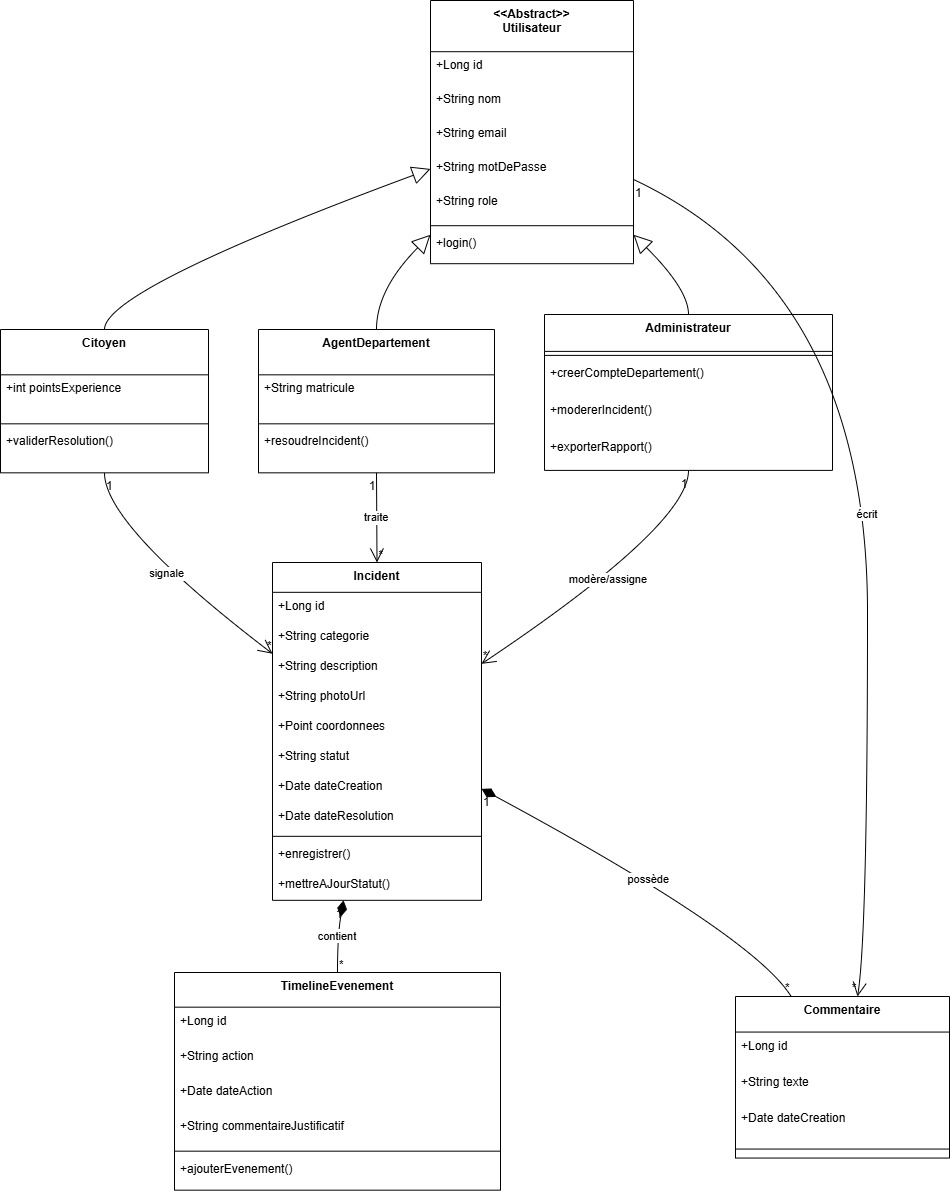
\includegraphics[width=0.9\textwidth]{classes_global.jpg}
    \caption{Diagramme de classes global initial}
    \label{fig:classes_global}
\end{figure}

\section*{Conclusion}
\addcontentsline{toc}{section}{Conclusion}
Ce deuxième chapitre nous a permis de structurer la planification agile du projet en identifiant l'équipe SCRUM, en découpant le projet en Sprints opérationnels, et en formalisant le Backlog de produit. Nous avons également établi la modélisation fonctionnelle et conceptuelle globale de \textit{SafeCity-Connect}. Le chapitre suivant détaillera le Sprint 0, consacré à la mise en place de notre architecture logicielle et de nos outils de développement.

\newpage

% Chapitre 3 : Sprint 0 -- Architecture logicielle et Outils de développement
% ==============================================================================
% FICHIER : chapitre3.tex
% Description : Chapitre 3 (Sprint 0) : Architecture logicielle et Framework de développement
% Auteurs : Dhia Fersi & Mohamed Iyed Amiri (ISET Bizerte)
% Organisme d'accueil : HRMAPS
% ==============================================================================

\chapter[Sprint 0 : Architecture et Outils]{Sprint 0 : Architecture logicielle et Framework de développement}

\section*{Introduction}
\addcontentsline{toc}{section}{Introduction}
Le Sprint 0 constitue le point de départ technique de notre projet de développement. Il a pour but de définir les choix d'architecture logicielle, de préparer l'infrastructure réseau et sécurité, d'harmoniser les outils de développement et de configurer l'ensemble des environnements matériels et logiciels. Ce chapitre présente le Backlog du Sprint 0, détaille la vue architecturale de \textit{SafeCity-Connect} (comprenant l'architecture de sécurité OAuth2/OIDC) et dresse l'état des outils et frameworks retenus pour la réalisation du projet.

% ------------------------------------------------------------------------------
% 1. BACKLOG SPRINT 0
% ------------------------------------------------------------------------------
\section{Backlog Sprint 0}
Le Sprint 0 vise à poser les jalons technologiques indispensables avant d'entamer les sprints de développement fonctionnels. Ses objectifs opérationnels se résument à :
\begin{itemize}
    \item \textbf{Configurer le dépôt Git} et le workflow de branchement de l'équipe.
    \item \textbf{Orchestrer l'infrastructure locale} via Docker et Docker Compose (base de données, Keycloak, microservice IA).
    \item \textbf{Initialiser les projets squelettes} (Backend Spring Boot, Web Admin Angular, et App Mobile Flutter).
    \item \textbf{Valider l'interfaçage initial} entre tous ces systèmes.
\end{itemize}

% ------------------------------------------------------------------------------
% 2. VUE ARCHITECTURALE DU SYSTÈME
% ------------------------------------------------------------------------------
\section{Vue architecturale du système}

\subsection{Architecture globale du système}
Pour garantir la flexibilité, le découplage des responsabilités et la robustesse de notre plateforme, nous avons conçu une architecture client-serveur multiniveaux articulée autour de 5 couches interdépendantes :
\begin{enumerate}
    \item \textbf{Le Client Web (Angular 18)} : Fournit la console d'administration municipale pour le suivi de la Heatmap, la modération, la gestion des rôles Keycloak et les exports analytiques.
    \item \textbf{Le Client Mobile (Flutter)} : L'application mobile multiplateforme destinée aux citoyens (signalement avec photo, commentaires, statut de résolution, notation des correctifs) et aux agents techniques (visualisation des missions et transmission de la photo preuve de fixation).
    \item \textbf{Le Serveur de Sécurité (Keycloak)} : Centralise l'authentification unifiée (SSO) et le contrôle d'accès basé sur les rôles.
    \item \textbf{L'API Gateway / Serveur Applicatif (Spring Boot 3.2)} : Gère les contrôles métiers, les services d'alertes e-mail et coordonne les flux de données.
    \item \textbf{La Base de Données (PostgreSQL / PostGIS)} : Assure le stockage relationnel et l'indexation cartographique spatiale native.
    \item \textbf{Le Microservice d'IA (Python YOLO)} : Traite l'analyse visuelle des photos chargées.
\end{enumerate}

La figure \ref{fig:schema_architecture} représente graphiquement cette organisation système.

\begin{figure}[H]
    \centering
    \framebox[\textwidth]{\vbox to 6cm{\vfill\hbox to \textwidth{\hss\textbf{[Figure : Schéma d'Architecture Système Globale]}\hss}\vfill}}
    \caption{Architecture globale de SafeCity-Connect}
    \label{fig:schema_architecture}
\end{figure}

\subsection{Architecture logicielle du système}
L'architecture de sécurité repose sur les standards de l'industrie pour les applications web monopages (SPA) :
\begin{itemize}
    \item \textbf{OAuth2 et OpenID Connect (OIDC)} : protocoles de référence pour déléguer l'authentification et l'autorisation de manière sécurisée.
    \item \textbf{Flux PKCE (Proof Key for Code Exchange)} : Utilisé lors de l'authentification côté frontend Angular pour interagir de manière ultra-sécurisée avec Keycloak sans requérir le stockage d'un secret client dans le code du navigateur.
    \item \textbf{Validation JWT} : Le frontend transmet le jeton d'accès JWT dans l'en-tête HTTP \texttt{Authorization: Bearer <JWT>} à chaque appel API. Le backend Spring Boot valide ce jeton cryptographiquement à l'aide des clés publiques de Keycloak, garantissant l'intégrité et la confidentialité des requêtes.
\end{itemize}

% ------------------------------------------------------------------------------
% 3. PRÉSENTATION DES OUTILS DE DÉVELOPPEMENT
% ------------------------------------------------------------------------------
\section{Présentation des outils de développement}

\subsection{Environnement Matériel}
Le développement et les tests locaux ont été menés sur des postes de travail équipés de processeurs multicœurs (Intel Core i7, 16 Go de RAM, disques SSD rapides) indispensables pour exécuter simultanément les multiples conteneurs Docker (Keycloak, PostgreSQL, Spring Boot, Angular, YOLO AI).

\subsection{Environnement Logiciel}
L'environnement logiciel comprend les outils de productivité et de conteneurisation suivants :
\begin{itemize}
    \item \textbf{Système d'Exploitation} : Windows 11 Professionnel.
    \item \textbf{IDEs} : \textbf{IntelliJ IDEA Ultimate} (développement Java/Spring Boot) et \textbf{Visual Studio Code / Android Studio} (développement TypeScript/Angular et mobile Flutter).
    \item \textbf{Orchestration Docker \& Docker Compose} : Essentiel pour packager et déployer instantanément tous nos services dans des conteneurs isolés et reproductibles.
    \item \textbf{Gestion des Versions} : \textbf{Git} combiné à l'hébergeur \textbf{GitHub}.
\end{itemize}

\subsection{Langage et Framework de développement}
Le tableau \ref{tab:sprint0_technologies} résume les frameworks et technologies retenus :

\begin{table}[H]
    \centering
    \caption{Frameworks et Technologies choisis}
    \label{tab:sprint0_technologies}
    \vspace{0.3cm}
    \begin{tabularx}{\textwidth}{l X}
        \toprule
        \textbf{Framework / Langage} & \textbf{Justification du Choix} \\
        \midrule
        \textbf{Java 21} & Version LTS offrant des performances accrues (Virtual Threads, Pattern Matching). \\
        \textbf{Spring Boot 3.2} & Framework backend de référence en Java, gérant la sécurité (OAuth2) et Spring Data JPA. \\
        \textbf{Angular 18} & Framework web robuste pour le dashboard d'administration réactif de la municipalité. \\
        \textbf{Flutter 3.x / Dart} & Framework mobile de Google pour compiler nativement l'application citoyen et agent de terrain sur Android et iOS. \\
        \textbf{PostgreSQL / PostGIS} & SGBD relationnel robuste doté de la meilleure extension spatiale pour stocker la géo-localisation. \\
        \textbf{Python / YOLO} & Écosystème leader pour la détection et classification automatique d'images. \\
        \bottomrule
    \end{tabularx}
\end{table}

\section*{Conclusion}
\addcontentsline{toc}{section}{Conclusion}
Le Sprint 0 s'est achevé avec succès. Nous avons défini l'architecture multiniveau sécurisée de \textit{SafeCity-Connect}, installé les environnements de développement et validé l'empilement technologique choisi. Forts de cette infrastructure technique opérationnelle, nous pouvons aborder le premier sprint fonctionnel présenté dans le chapitre suivant, dédié à la gestion des comptes, de l'authentification unifiée et de la sécurité des utilisateurs.

\newpage

% Chapitre 4 : Sprint 1 -- Inscription, Authentification, Gestion profil
% ==============================================================================
% FICHIER : chapitre4.tex
% Description : Chapitre 4 (Sprint 1) : Inscription, Authentification, Gestion profil
% Auteurs : Dhia Fersi & Mohamed Iyed Amiri (ISET Bizerte)
% Organisme d'accueil : HRMAPS
% ==============================================================================

\chapter[Sprint 1 : Authentification et Profil]{Sprint 1 : Inscription, Authentification, Gestion profil et réinitialiser mot de passe}

\section*{Introduction}
\addcontentsline{toc}{section}{Introduction}
La gestion d'identité et la sécurité constituent le premier pilier fonctionnel de la plateforme \textit{SafeCity-Connect}. L'objectif du Sprint 1 est de concevoir et réaliser un système d'authentification robuste et unifié, permettant aux citoyens de s'inscrire, de se connecter, de gérer leurs données de profil et de réinitialiser leur mot de passe en toute sécurité. Ce chapitre détaille l'analyse fonctionnelle, les diagrammes de séquence UML, le diagramme de classes spécifique au sprint, et la réalisation technique s'appuyant sur Keycloak et Spring Security.

% ------------------------------------------------------------------------------
% 1. BACKLOG SPRINT 1
% ------------------------------------------------------------------------------
\section{BACKLOG Sprint 1}
Le Backlog du Sprint 1 regroupe l'ensemble des récits utilisateurs associés à la gestion d'identité :
\begin{itemize}
    \item \textbf{US02 -- Inscription et Connexion SSO} : Permettre à un citoyen de créer un compte et de se connecter de manière centralisée.
    \item \textbf{US03 -- Gestion de profil et Mot de passe oublié} : Permettre à l'utilisateur connecté de modifier ses données personnelles et de réinitialiser son mot de passe en cas de perte via e-mail.
\end{itemize}

% ------------------------------------------------------------------------------
% 2. ANALYSE ET SPÉCIFICATION DES BESOINS
% ------------------------------------------------------------------------------
\section{Analyse et spécification des besoins}

\subsection{Diagramme de cas d'utilisation}
La figure \ref{fig:uc_sprint1} modélise les cas d'utilisation spécifiques aux comptes utilisateurs.

\begin{figure}[H]
    \centering
    \framebox[\textwidth]{\vbox to 5.5cm{\vfill\hbox to \textwidth{\hss\textbf{[Figure : Diagramme de Cas d'Utilisation -- Sprint 1 (Gestion Comptes)]}\hss}\vfill}}
    \caption{Diagramme de cas d'utilisation : Sprint 1}
    \label{fig:uc_sprint1}
\end{figure}

\subsection{Description textuelle}
Voici la description textuelle du cas d'utilisation principal \textbf{« S'authentifier »} :
\begin{itemize}
    \item \textbf{Acteurs} : Citoyen, Administrateur.
    \item \textbf{Préconditions} : L'acteur possède un compte enregistré dans le système.
    \item \textbf{Scénario nominal} :
    \begin{enumerate}
        \item L'utilisateur clique sur le bouton « Connexion » de l'application Angular.
        \item L'application redirige l'utilisateur vers la page de login Keycloak sécurisée.
        \item L'utilisateur saisit son identifiant (ou email) et son mot de passe, puis valide.
        \item Keycloak valide les informations d'identification.
        \item Keycloak redirige l'utilisateur vers le frontend avec un code d'autorisation.
        \item Le frontend échange ce code contre un jeton JWT d'accès et un jeton de rafraîchissement.
        \item L'utilisateur accède à son espace personnel.
    \end{enumerate}
    \item \textbf{Scénarios alternatifs} : En cas d'identifiants incorrects, un message d'erreur s'affiche sur la mire Keycloak et l'authentification est rejetée.
\end{itemize}

% ------------------------------------------------------------------------------
% 3. PRÉSENTATION ÉCRAN IHM
% ------------------------------------------------------------------------------
\section{Présentation Écran IHM}
Les interfaces utilisateurs de ce sprint ont été conçues pour être fluides et claires, respectant la charte graphique moderne et adaptative de \textit{SafeCity-Connect}.

\begin{figure}[H]
    \centering
    \framebox[\textwidth]{\vbox to 6cm{\vfill\hbox to \textwidth{\hss\textbf{[Capture d'écran : Interface d'Authentification Keycloak SSO personnalisée]}\hss}\vfill}}
    \caption{Mire de connexion sécurisée (Keycloak SSO)}
    \label{fig:ihm_login}
\end{figure}

% ------------------------------------------------------------------------------
% 4. DIAGRAMME DE SÉQUENCE
% ------------------------------------------------------------------------------
\section{Diagramme de séquence}
Cette section illustre la cinématique des messages échangés entre le client Angular, Keycloak, le backend Spring Boot et la base de données PostgreSQL pour les différents cas d'utilisation.

\subsection{Diagramme de séquence « Authentification »}
La figure \ref{fig:seq_auth} décrit le flux d'authentification s'appuyant sur le protocole OpenID Connect et le protocole PKCE.

\begin{figure}[H]
    \centering
    \framebox[\textwidth]{\vbox to 6cm{\vfill\hbox to \textwidth{\hss\textbf{[Diagramme de Séquence UML : Authentification PKCE OIDC]}\hss}\vfill}}
    \caption{Diagramme de séquence : Authentification unifiée}
    \label{fig:seq_auth}
\end{figure}

\subsection{Diagramme de séquence « Gestion profil »}
La figure \ref{fig:seq_profile} illustre le cas où l'utilisateur connecté met à jour son profil (ex : prénom, nom, email).

\begin{figure}[H]
    \centering
    \framebox[\textwidth]{\vbox to 5.5cm{\vfill\hbox to \textwidth{\hss\textbf{[Diagramme de Séquence UML : Mise à jour du Profil]}\hss}\vfill}}
    \caption{Diagramme de séquence : Gestion du profil utilisateur}
    \label{fig:seq_profile}
\end{figure}

\subsection{Diagramme de séquence « Inscription »}
La figure \ref{fig:seq_inscription} montre comment le compte citoyen est créé dans Keycloak et synchronisé en base de données.

\begin{figure}[H]
    \centering
    \framebox[\textwidth]{\vbox to 5.5cm{\vfill\hbox to \textwidth{\hss\textbf{[Diagramme de Séquence UML : Inscription Citoyenne et Synchro BDD]}\hss}\vfill}}
    \caption{Diagramme de séquence : Inscription d'un nouveau compte}
    \label{fig:seq_inscription}
\end{figure}

\subsection{Diagramme de séquence « mot de passe oublier »}
La figure \ref{fig:seq_pwd_forget} montre le processus de réinitialisation sécurisé par envoi d'un e-mail contenant un lien temporaire signé.

\begin{figure}[H]
    \centering
    \framebox[\textwidth]{\vbox to 5.5cm{\vfill\hbox to \textwidth{\hss\textbf{[Diagramme de Séquence UML : Mot de passe oublié et Réinitialisation]}\hss}\vfill}}
    \caption{Diagramme de séquence : Réinitialisation du mot de passe}
    \label{fig:seq_pwd_forget}
\end{figure}

% ------------------------------------------------------------------------------
% 5. DIAGRAMME DE CLASSES
% ------------------------------------------------------------------------------
\section{Diagramme de classes}
La structure de données de ce sprint gère l'utilisateur et son profil. Le diagramme de classes est illustré dans la figure \ref{fig:class_sprint1}.

\begin{figure}[H]
    \centering
    \framebox[\textwidth]{\vbox to 5.5cm{\vfill\hbox to \textwidth{\hss\textbf{[Figure : Diagramme de Classes -- Sprint 1 (Gestion Utilisateurs)]}\hss}\vfill}}
    \caption{Diagramme de classes du Sprint 1}
    \label{fig:class_sprint1}
\end{figure}

% ------------------------------------------------------------------------------
% 6. RÉALISATION
% ------------------------------------------------------------------------------
\section{Réalisation}

\subsection{Création du schéma « user »}
La table correspondante dans notre base de données relationnelle est \texttt{table_user_profile}. Elle est déclarée avec les attributs \texttt{id} (UUID hérité de Keycloak), \texttt{username}, \texttt{email}, et \texttt{impact_points} (valeur initiale à 0).

\subsection{Sécurité}
La sécurité est orchestrée en couplant notre serveur d'identité Keycloak avec la configuration de sécurité Spring Security de notre application backend.

\paragraph{Configuration Keycloak}
Nous avons créé un Realm nommé \texttt{safecity} au sein de Keycloak. Dans ce Realm, trois rôles de base sont configurés :
\begin{itemize}
    \item \textbf{CITIZEN} : Attribué par défaut à tout utilisateur s'inscrivant via le formulaire public.
    \item \textbf{ADMIN} : Attribué manuellement aux gestionnaires municipaux.
    \item \textbf{DEPARTMENT} : Attribué aux agents techniques et départements municipaux chargés des travaux.
\end{itemize}
Nous avons également configuré un client public \texttt{safecity-frontend} supportant le flux OAuth2 PKCE avec redirections autorisées vers l'adresse \texttt{http://localhost:4200}.

\paragraph{Configuration Spring Security}
Côté Spring Boot 3.2, nous configurons l'application en tant que serveur de ressources OAuth2 (\textit{OAuth2 Resource Server}) dans une classe de configuration de sécurité :
\begin{verbatim}
@Bean
public SecurityFilterChain securityFilterChain(HttpSecurity http) throws Exception {
    http
        .authorizeHttpRequests(auth -> auth
            .requestMatchers("/api/public/**").permitAll()
            .requestMatchers("/api/admin/**").hasRole("ADMIN")
            .requestMatchers("/api/department/**").hasRole("DEPARTMENT")
            .requestMatchers("/api/citizen/**").hasRole("CITIZEN")
            .anyRequest().authenticated()
        )
        .oauth2ResourceServer(oauth2 -> oauth2.jwt(Customizer.withDefaults()));
    return http.build();
}
\end{verbatim}

\subsection{Création des web services « API Endpoint »}
Les services web exposés sont développés sous forme de contrôleurs REST Spring Boot. Par exemple, le contrôleur \texttt{UserProfileController} expose les routes permettant de récupérer et de modifier les données de profil :
\begin{itemize}
    \item \textbf{GET} \texttt{/api/citizen/profile} : Récupérer les informations de l'utilisateur connecté (id extrait à partir du JWT).
    \item \textbf{PUT} \texttt{/api/citizen/profile} : Mettre à jour les informations (nom, prénom) et synchroniser avec Keycloak via l'API d'administration Keycloak.
\end{itemize}

\subsection{Enchaînement des interfaces réalisées}
Lors de l'utilisation réelle, un utilisateur non authentifié arrivant sur l'application Angular est immédiatement redirigé vers l'IHM de Keycloak. Dès la saisie d'identifiants valides, l'enchaînement des interfaces le ramène vers la page d'accueil d'historique de signalement citoyen où ses informations de profil (nom, points d'impact) s'affichent de manière personnalisée.

\section*{Conclusion}
Le Sprint 1 s'est achevé avec la réalisation complète de notre brique de sécurité et de gestion d'identité. Grâce à l'intégration robuste de Keycloak et Spring Security, la plateforme \textit{SafeCity-Connect} garantit la confidentialité des données et sépare hermétiquement les fonctionnalités citoyennes et d'administration. Le chapitre suivant présentera le Sprint 2, le cœur de l'expérience citoyenne, centré sur la gestion des signalements d'incidents sur le terrain assistée par l'intelligence artificielle.

\newpage

% Chapitre 5 : Sprint 2 -- Gestion des Signalements et Analyse IA
% ==============================================================================
% FICHIER : chapitre5.tex
% Description : Chapitre 5 (Sprint 2) : Gestion des Signalements et Analyse IA
% Auteurs : Dhia Fersi & Mohamed Iyed Amiri (ISET Bizerte)
% Organisme d'accueil : HRMAPS
% ==============================================================================

\chapter[Sprint 2 : Signalements et IA]{Sprint 2 : Gestion des Signalements et Analyse IA}

\section*{Introduction}
\addcontentsline{toc}{section}{Introduction}
La remontée précise, rapide et géo-localisée des anomalies urbaines est l'activité centrale des citoyens sur notre plateforme. L'objectif du Sprint 2 est de réaliser le processus complet de signalement d'un incident depuis le terrain. Pour simplifier l'expérience utilisateur et automatiser la qualification du signalement, nous intégrons un module d'Intelligence Artificielle de détection d'objets (YOLO AI) qui analyse la photo de l'anomalie pour en déduire automatiquement sa catégorie. Ce chapitre présente l'analyse de ce sprint, les diagrammes UML correspondants, et l'implémentation de la cartographie Leaflet, d'Hibernate Spatial (PostGIS) et de l'interfaçage avec l'IA.

% ------------------------------------------------------------------------------
% 1. BACKLOG SPRINT 2
% ------------------------------------------------------------------------------
\section{BACKLOG Sprint 2}
Le Backlog du Sprint 2 se concentre sur les fonctionnalités opérationnelles de signalement mobile :
\begin{itemize}
    \item \textbf{US04 -- Signalement d'incident géo-localisé (Citoyen)} : Permettre d'ouvrir la carte mobile Flutter, d'y pointer la position via GPS, de capturer une photo, d'obtenir le classement IA et d'ajouter des commentaires de départ.
    \item \textbf{US05 -- Consultation de l'état sur la carte (Citoyen)} : Permettre au citoyen de visualiser sur la carte interactive l'état actuel de l'incident (signalé, en cours, réparé).
\end{itemize}

% ------------------------------------------------------------------------------
% 2. ANALYSE ET SPÉCIFICATION DES BESOINS
% ------------------------------------------------------------------------------
\section{Analyse et spécification des besoins}

\subsection{Diagramme de cas d'utilisation}
La figure \ref{fig:uc_sprint2} illustre le cas d'utilisation détaillé de signalement d'incident.

\begin{figure}[H]
    \centering
    \framebox[\textwidth]{\vbox to 5.5cm{\vfill\hbox to \textwidth{\hss\textbf{[Figure : Diagramme de Cas d'Utilisation -- Sprint 2 (Signalement)]}\hss}\vfill}}
    \caption{Diagramme de cas d'utilisation : Sprint 2}
    \label{fig:uc_sprint2}
\end{figure}

\subsection{Description textuelle}
Voici la description textuelle du cas d'utilisation principal \textbf{« Signaler un incident »} :
\begin{itemize}
    \item \textbf{Acteur} : Citoyen.
    \item \textbf{Préconditions} : L'acteur est connecté à son compte citoyen sur l'application.
    \item \textbf{Scénario nominal} :
    \begin{enumerate}
        \item Le citoyen ouvre l'application mobile Flutter et clique sur « Signaler un incident ».
        \item L'application affiche la carte interactive Leaflet et géolocalise l'utilisateur via le GPS de son téléphone.
        \item Le citoyen capture la photo de l'anomalie directement depuis l'appareil photo du smartphone.
        \item Le client mobile envoie l'image au backend Spring Boot, qui la transfère instantanément au service YOLO AI.
        \item Le service YOLO AI renvoie la classe détectée (ex : Nid-de-poule).
        \item Le citoyen prend connaissance du choix de l'IA (qu'il peut modifier au besoin), ajoute un commentaire initial et valide le signalement.
        \item Le backend enregistre l'incident, initialise la **timeline d'évolution**, et déclenche une alerte de notification e-mail automatique à destination de l'administrateur municipal.
    \end{enumerate}
    \item \textbf{Scénarios alternatifs} : Si le microservice d'IA YOLO est indisponible, le système affiche un message d'avertissement et invite l'utilisateur à sélectionner lui-même manuellement la catégorie de l'incident dans une liste déroulante.
\end{itemize}

% ------------------------------------------------------------------------------
% 3. PRÉSENTATION ÉCRAN IHM
% ------------------------------------------------------------------------------
\section{Présentation écran IHM}
L'interface de signalement a été particulièrement optimisée pour une utilisation sur smartphone :

\begin{figure}[H]
    \centering
    \framebox[\textwidth]{\vbox to 6.5cm{\vfill\hbox to \textwidth{\hss\textbf{[Capture d'écran : Formulaire de Signalement Citoyen responsive avec carte Leaflet]}\hss}\vfill}}
    \caption{Interface de signalement mobile-first}
    \label{fig:ihm_report}
\end{figure}

% ------------------------------------------------------------------------------
% 4. DIAGRAMME DE SÉQUENCE
% ------------------------------------------------------------------------------
\section{Diagramme de séquence}
La figure \ref{fig:seq_sprint2} illustre l'interaction de signalement citoyen intégrant l'analyse d'image automatique.

\begin{figure}[H]
    \centering
    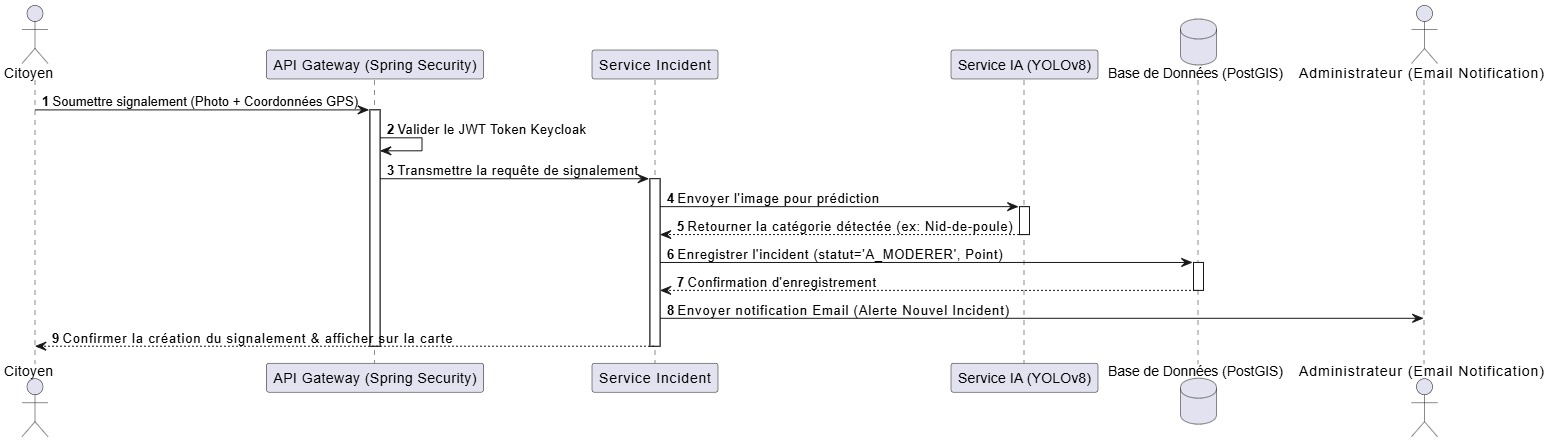
\includegraphics[width=\textwidth]{seq_signalement_yolo.jpg}
    \caption{Diagramme de séquence : Processus de signalement avec YOLO}
    \label{fig:seq_sprint2}
\end{figure}

% ------------------------------------------------------------------------------
% 5. DIAGRAMME DE CLASSES
% ------------------------------------------------------------------------------
\section{Diagramme de classes}
La figure \ref{fig:class_sprint2} montre le modèle structurel gérant l'incident, sa catégorie et sa géolocalisation.

\begin{figure}[H]
    \centering
    \framebox[\textwidth]{\vbox to 5.5cm{\vfill\hbox to \textwidth{\hss\textbf{[Figure : Diagramme de Classes -- Sprint 2 (Signalement et Données Spatiales)]}\hss}\vfill}}
    \caption{Diagramme de classes du Sprint 2}
    \label{fig:class_sprint2}
\end{figure}

% ------------------------------------------------------------------------------
% 6. RÉALISATION
% ------------------------------------------------------------------------------
\section{Réalisation}

\subsection{Intégration d'Hibernate Spatial et PostGIS}
Pour stocker et manipuler les coordonnées GPS géospatiales de manière native sous Spring Boot 3.2, nous intégrons la dépendance \texttt{hibernate-spatial}. Celle-ci étend les fonctionnalités standards de JPA/Hibernate pour supporter les types de la bibliothèque JTS (\textit{Java Topology Suite}) :

\begin{verbatim}
@Entity
@Table(name = "table_incident")
public class Incident {
    @Id
    @GeneratedValue(strategy = GenerationType.IDENTITY)
    private Long id;
    
    private String description;
    private String status;
    private String photoUrl;
    
    // Type géographique Point géré nativement par PostGIS
    private Point geom; 
    
    @ManyToOne
    @JoinColumn(name = "category_id")
    private Category category;
}
\end{verbatim}

\subsection{Intégration de la carte Leaflet}
Côté frontend mobile Flutter, nous utilisons le package \textbf{flutter\_map} (couche d'interfaçage avec Leaflet.js). L'application charge des tuiles géographiques cartographiques en mode sombre (\textit{Dark Matter}) de CartoDB, assurant une esthétique premium et reposante. Le citoyen définit l'emplacement de l'incident grâce à un marqueur tactile interactif, transmettant les coordonnées (longitude/latitude) au format standard WGS 84.

\subsection{Microservice IA YOLO}
Le backend Spring Boot communique de manière asynchrone avec un microservice écrit en Python et basé sur le framework léger FastAPI. Ce service expose une API REST de traitement d'images. À la réception de l'image chargée, le service charge un modèle de détection d'objets YOLO pré-entraîné, isole l'anomalie détectée, calcule un score de confiance (ex : $0.94$ pour un nid-de-poule), et retourne la catégorie correspondante au format JSON au backend :
\begin{verbatim}
{
  "class_name": "Nid-de-poule",
  "confidence": 0.94,
  "status": "SUCCESS"
}
\end{verbatim}

\subsection{Enchaînement des interfaces réalisées}
Sur le terrain, l'utilisateur ouvre l'application, clique sur la carte Leaflet pour localiser un incident, et appuie sur « Prendre Photo ». La photo est capturée via la caméra de l'appareil mobile, transférée au serveur, et analysée instantanément. La catégorie s'affiche sous forme de badge vert pour confirmation finale avant soumission définitive.

\section*{Conclusion}
Le Sprint 2 a permis de réaliser le cœur opérationnel de la plateforme \textit{SafeCity-Connect} pour l'expérience citoyenne. Grâce au couplage de Leaflet, Hibernate Spatial et de l'analyse automatisée par l'intelligence artificielle YOLO, la saisie d'un incident prend moins de 30 secondes pour un utilisateur sur son mobile. Le chapitre suivant détaillera le Sprint 3, qui conçoit et implémente les fonctionnalités administratives d'aide à la décision communale.

\newpage

% Chapitre 6 : Sprint 3 -- Espace Administration, Heatmap et Statistiques
% ==============================================================================
% FICHIER : chapitre6.tex
% Description : Chapitre 6 (Sprint 3) : Espace Administration, Heatmap et Statistiques
% Auteurs : Dhia Fersi & Mohamed Iyed Amiri (ISET Bizerte)
% Organisme d'accueil : HRMAPS
% ==============================================================================

\chapter[Sprint 3 : Administration et Heatmap]{Sprint 3 : Espace Administration, Heatmap et Statistiques}

\section*{Introduction}
\addcontentsline{toc}{section}{Introduction}
Une gestion de voirie efficace requiert des outils d'analyse puissants pour aider les décideurs municipaux à prioriser les chantiers et à suivre l'évolution des résolutions. L'objectif du Sprint 3 est de réaliser l'espace d'administration de la plateforme \textit{SafeCity-Connect}. Cet espace fournit aux administrateurs municipaux un portail web décisionnel (Angular 18) pour affecter les interventions aux départements techniques, suivre la carte thermique (\textit{Heatmap}), recevoir des alertes par e-mail lors de nouveaux signalements, et exporter des analyses hebdomadaires ou des fiches d'incidents au format PDF. Ce chapitre présente le backlog, l'analyse fonctionnelle, les modélisations UML, et l'implémentation des services de notifications, de cartographie et de génération de rapports.

% ------------------------------------------------------------------------------
% 1. BACKLOG SPRINT 3
% ------------------------------------------------------------------------------
\section{BACKLOG Sprint 3}
Le Backlog du Sprint 3 cible les capacités de modération, d'analyse et d'alerte de l'administration :
\begin{itemize}
    \item \textbf{US06 -- Affectation aux départements (Admin)} : Permettre à l'administrateur d'affecter un incident validé à un département technique spécifique en créant une tâche d'intervention.
    \item \textbf{US07 -- Carte thermique et Exports analytiques (Admin)} : Permettre de visualiser la Heatmap PostGIS, d'exporter le récapitulatif hebdomadaire des anomalies (Excel/CSV) et de générer un rapport PDF complet de synthèse d'un incident.
    \item \textbf{US08 -- Alertes par E-mail (Admin)} : Configurer le service de messagerie pour avertir automatiquement l'administrateur par courriel lors de chaque nouveau signalement citoyen.
\end{itemize}

% ------------------------------------------------------------------------------
% 2. ANALYSE ET SPÉCIFICATION DES BESOINS
% ------------------------------------------------------------------------------
\section{Analyse et spécification des besoins}

\subsection{Diagramme de cas d'utilisation}
La figure \ref{fig:uc_sprint3} illustre les cas d'utilisation liés à l'affectation, aux alertes e-mail et aux fonctions d'export documentaires de l'Administrateur.

\begin{figure}[H]
    \centering
    \framebox[\textwidth]{\vbox to 5.5cm{\vfill\hbox to \textwidth{\hss\textbf{[Figure : Diagramme de Cas d'Utilisation -- Sprint 3 (Administration)]}\hss}\vfill}}
    \caption{Diagramme de cas d'utilisation : Sprint 3}
    \label{fig:uc_sprint3}
\end{figure}

\subsection{Description textuelle}
Voici la description textuelle du cas d'utilisation \textbf{« Exporter le rapport PDF d'un incident »} :
\begin{itemize}
    \item \textbf{Acteur} : Administrateur.
    \item \textbf{Préconditions} : L'incident sélectionné possède un historique d'actions (timeline).
    \item \textbf{Scénario nominal} :
    \begin{enumerate}
        \item L'administrateur consulte la fiche d'un incident sur le dashboard Angular.
        \item Il clique sur le bouton « Exporter Rapport PDF ».
        \item Le frontend envoie une requête vers l'API backend Spring Boot avec l'identifiant de l'incident.
        \item Le backend extrait les données de l'incident (localisation, catégorie, dates, acteur citoyen, agent technique affecté, photos avant/après, commentaires et historique d'états de la timeline).
        \item Le backend injecte ces données dans un template HTML via Thymeleaf, puis génère le document PDF.
        \item Le fichier PDF est renvoyé sous forme de flux binaire au navigateur.
        \item Le navigateur télécharge automatiquement le rapport PDF officiel.
    \end{enumerate}
    \item \textbf{Scénarios alternatifs} : En cas d'erreur de base de données, un message d'alerte s'affiche sur le dashboard de l'Admin et l'action est annulée.
\end{itemize}

% ------------------------------------------------------------------------------
% 3. PRÉSENTATION ÉCRAN IHM
% ------------------------------------------------------------------------------
\section{Présentation écran IHM}
L'interface de l'administrateur intègre la Heatmap et les contrôles d'export décisionnels :

\begin{figure}[H]
    \centering
    \framebox[\textwidth]{\vbox to 6.5cm{\vfill\hbox to \textwidth{\hss\textbf{[Capture d'écran : Console Admin Web -- Heatmap PostGIS et Menu d'Export PDF/Excel]}\hss}\vfill}}
    \caption{Interface du Tableau de bord d'Administration}
    \label{fig:ihm_admin}
\end{figure}

% ------------------------------------------------------------------------------
% 4. DIAGRAMME DE SÉQUENCE
% ------------------------------------------------------------------------------
\section{Diagramme de séquence}
La figure \ref{fig:seq_sprint3} montre les cinématiques d'appels lors de l'exportation d'une fiche d'anomalie au format PDF et de l'envoi de l'alerte e-mail lors de la création de l'incident.

\begin{figure}[H]
    \centering
    \framebox[\textwidth]{\vbox to 7.5cm{\vfill\hbox to \textwidth{\hss\textbf{[Diagramme de Séquence UML : Envoi d'Alerte E-mail et Export de Rapport PDF]}\hss}\vfill}}
    \caption{Diagramme de séquence : Notifications et Exports}
    \label{fig:seq_sprint3}
\end{figure}

% ------------------------------------------------------------------------------
% 5. DIAGRAMME DE CLASSES
% ------------------------------------------------------------------------------
\section{Diagramme de classes}
La figure \ref{fig:class_sprint3} présente le modèle structurel enrichi avec les relations de Département et de logs de notifications.

\begin{figure}[H]
    \centering
    \framebox[\textwidth]{\vbox to 5.5cm{\vfill\hbox to \textwidth{\hss\textbf{[Figure : Diagramme de Classes -- Sprint 3 (Admin \& Services tiers)]}\hss}\vfill}}
    \caption{Diagramme de classes du Sprint 3}
    \label{fig:class_sprint3}
\end{figure}

% ------------------------------------------------------------------------------
% 6. RÉALISATION
% ------------------------------------------------------------------------------
\section{Réalisation}

\subsection{Service d'Alertes par E-mail}
Dès qu'un citoyen soumet un signalement d'anomalie, la couche service Spring Boot intercepte l'événement de création et sollicite le composant \texttt{EmailNotificationService} (s'appuyant sur \texttt{spring-boot-starter-mail}) :
\begin{verbatim}
@Service
public class EmailNotificationService {
    @Autowired
    private JavaMailSender mailSender;

    public void sendIncidentAlertToAdmin(Incident incident) {
        SimpleMailMessage message = new SimpleMailMessage();
        message.setTo("admin@safecity.tn");
        message.setSubject("🚨 SafeCity-Connect : Nouveau signalement d'incident");
        message.setText("Un nouvel incident a été signalé !\n" +
                        "Catégorie : " + incident.getCategory().getLabel() + "\n" +
                        "Description : " + incident.getDescription() + "\n" +
                        "Coordonnées : " + ST_AsText(incident.getGeom()) + "\n" +
                        "Veuillez vous connecter pour affecter l'intervention.");
        mailSender.send(message);
    }
}
\end{verbatim}

\subsection{Génération du Rapport PDF de l'Incident}
Pour exporter la fiche d'incident en format PDF, nous utilisons la bibliothèque open-source **OpenPDF** (ou **iText**) au sein du backend. La classe \texttt{PdfExportService} génère dynamiquement un document structuré et paginé contenant :
\begin{itemize}
    \item L'en-tête officiel de la municipalité et le logo du projet.
    \item La fiche descriptive de l'anomalie et ses coordonnées cartographiques.
    \item La photo initiale de signalement et la photo preuve de fixation.
    \item Le fil de vie historique (**Timeline**) de l'incident.
    \item L'historique des commentaires rédigés par les citoyens.
\end{itemize}

\subsection{Export Hebdomadaire (Excel/CSV)}
Pour l'analyse quantitative, un service d'exportation de données interroge la base de données et écrit les incidents de la semaine écoulée dans un classeur Excel en exploitant la bibliothèque **Apache POI**. L'administrateur récupère ce fichier via l'API REST :
\texttt{GET /api/admin/incidents/export-weekly}.

\section*{Conclusion}
Le Sprint 3 dote la municipalité d'outils décisionnels et analytiques avancés. L'envoi automatique d'alertes e-mail garantit une réactivité immédiate dès le dépôt d'un signalement, tandis que l'affectation directe aux agents et les fonctionnalités d'export (Excel hebdomadaire, rapports PDF d'incidents) permettent d'archiver, de planifier et d'analyser scientifiquement l'entretien des quartiers. Le chapitre suivant traitera de l'étape de clôture par photo preuve de fixation et de la gamification.

\newpage

% Chapitre 7 : Sprint 4 -- Espace Gamification et Historique Citoyen
% ==============================================================================
% FICHIER : chapitre7.tex
% Description : Chapitre 7 (Sprint 4) : Espace Gamification, Clôture et Historique Citoyen
% Auteurs : Dhia Fersi & Mohamed Iyed Amiri (ISET Bizerte)
% Organisme d'accueil : HRMAPS
% ==============================================================================

\chapter[Sprint 4 : Gamification et Historique]{Sprint 4 : Espace Gamification, Clôture et Historique}

\section*{Introduction}
\addcontentsline{toc}{section}{Introduction}
La réussite d'une plateforme participative comme \textit{SafeCity-Connect} repose sur l'interaction active et transparente entre les citoyens, la municipalité et les services techniques. L'objectif du Sprint 4 est de finaliser le cycle de vie de l'incident. Ce cycle comprend le téléversement de la photo preuve par le département technique, la modération de cette preuve par l'administrateur (acceptation ou rejet motivé avec saisie obligatoire d'une raison), et la possibilité pour le citoyen de commenter et d'évaluer la qualité de la réparation (\textit{review fixes}). De plus, ce sprint implémente le suivi global par une frise chronologique détaillée (\textbf{Timeline}) pour chaque anomalie, réservée à la consultation de l'administrateur. Ce chapitre présente le backlog, la modélisation fonctionnelle, les diagrammes UML, et l'implémentation de la logique de clôture, de modération et de commentaires.

% ------------------------------------------------------------------------------
% 1. BACKLOG SPRINT 4
% ------------------------------------------------------------------------------
\section{BACKLOG Sprint 4}
Le Backlog du Sprint 4 consolide les récits utilisateurs liés aux chantiers, à la modération finale et aux retours citoyens :
\begin{itemize}
    \item \textbf{US09 -- Photo preuve de fixation (Département)} : Permettre à l'agent technique d'uploader une photo de l'anomalie réparée pour clore son intervention.
    \item \textbf{US10 -- Modération et Raison de Rejet (Admin)} : Permettre à l'administrateur de valider ou de refuser la réparation soumise par le département en saisissant une raison obligatoire enregistrée dans la timeline de l'incident.
    \item \textbf{US11 -- Commentaires et Notation de la réparation (Citoyen)} : Permettre aux citoyens d'écrire des commentaires sur l'incident et de donner leur avis après la résolution de l'anomalie (\textit{review fixes}).
\end{itemize}

% ------------------------------------------------------------------------------
% 2. ANALYSE ET SPÉCIFICATION DES BESOINS
% ------------------------------------------------------------------------------
\section{Analyse et spécification des besoins}

\subsection{Diagramme de cas d'utilisation}
La figure \ref{fig:uc_sprint4} présente les cas d'utilisation liés à l'authentification des agents, la modération des preuves de fixation, la rédaction de commentaires et l'attribution finale des points de gamification.

\begin{figure}[H]
    \centering
    \framebox[\textwidth]{\vbox to 5.5cm{\vfill\hbox to \textwidth{\hss\textbf{[Figure : Diagramme de Cas d'Utilisation -- Sprint 4 (Clôture et Avis Citoyens)]}\hss}\vfill}}
    \caption{Diagramme de cas d'utilisation : Sprint 4}
    \label{fig:uc_sprint4}
\end{figure}

\subsection{Description textuelle}
Voici la description textuelle du cas d'utilisation principal \textbf{« Modérer la résolution d'un incident »} :
\begin{itemize}
    \item \textbf{Acteur} : Administrateur.
    \item \textbf{Préconditions} : L'incident est à l'état « A\_VALIDER\_FIX » (le département technique a téléversé sa photo preuve).
    \item \textbf{Scénario nominal} :
    \begin{enumerate}
        \item L'administrateur ouvre l'interface de modération de la réparation sur la console web.
        \item Il compare la photo initiale (avant) et la photo preuve (après) fournie par les agents.
        \item \textbf{Cas A (Acceptation)} : L'administrateur valide la réparation. Le statut passe à « RESOLVED », la timeline est mise à jour, et le citoyen reçoit automatiquement ses points d'impact.
        \item \textbf{Cas B (Rejet)} : L'administrateur refuse la réparation, saisit obligatoirement un motif (ex : « Bitume mal tassé, fissure encore visible ») et valide. Le statut repasse à « EN\_COURS » pour ré-intervention, et la raison du refus est consignée dans la timeline de l'incident pour le suivi de l'administration.
    \end{enumerate}
    \item \textbf{Scénarios alternatifs} : Si l'administrateur valide l'incident sans saisir de motif en cas de rejet, le système affiche un message d'erreur et bloque la validation.
\end{itemize}

% ------------------------------------------------------------------------------
% 3. PRÉSENTATION ÉCRAN IHM
% ------------------------------------------------------------------------------
\section{Présentation écran IHM}
L'interface de l'application mobile Flutter permet aux citoyens de donner leur avis sur les réparations et d'échanger des commentaires :

\begin{figure}[H]
    \centering
    \framebox[\textwidth]{\vbox to 6.5cm{\vfill\hbox to \textwidth{\hss\textbf{[Capture d'écran : Application Flutter Citoyen -- Section Commentaires et Avis sur la Réparation (sans timeline)]}\hss}\vfill}}
    \caption{Interface de l'historique citoyen avec statut et commentaires}
    \label{fig:ihm_gamification}
\end{figure}

% ------------------------------------------------------------------------------
% 4. DIAGRAMME DE SÉQUENCE
% ------------------------------------------------------------------------------
\section{Diagramme de sequence}
La figure \ref{fig:seq_sprint4} décrit le flux d'informations lors du rejet d'une réparation par l'administrateur avec motif, sa mise à jour en base de données et sa consignation dans la timeline d'incident de l'administrateur.

\begin{figure}[H]
    \centering
    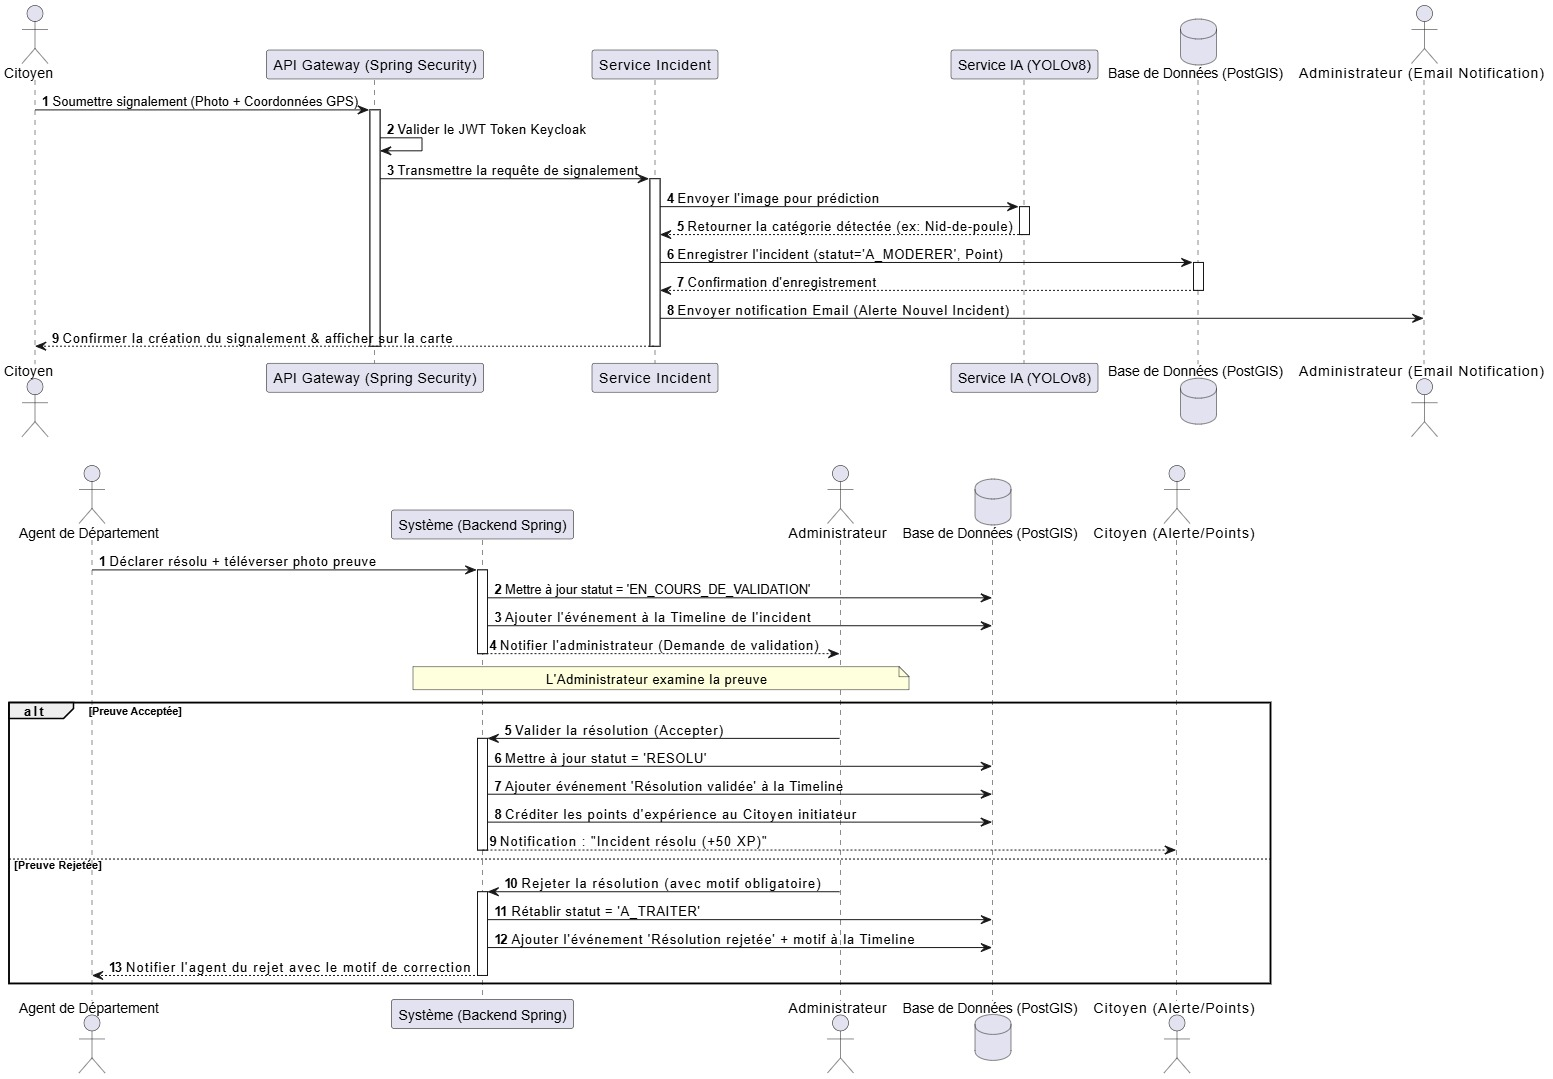
\includegraphics[width=\textwidth]{seq_resolution_moderation.jpg}
    \caption{Diagramme de séquence : Modération et Retours citoyens}
    \label{fig:seq_sprint4}
\end{figure}

% ------------------------------------------------------------------------------
% 5. DIAGRAMME DE CLASSES
% ------------------------------------------------------------------------------
\section{Diagramme de classes}
La figure \ref{fig:class_sprint4} détaille la structure statique du code gérant l'historique des statuts (Timeline), les entités de commentaires (\texttt{Comment}) et les notes d'évaluation (\texttt{FixReview}).

\begin{figure}[H]
    \centering
    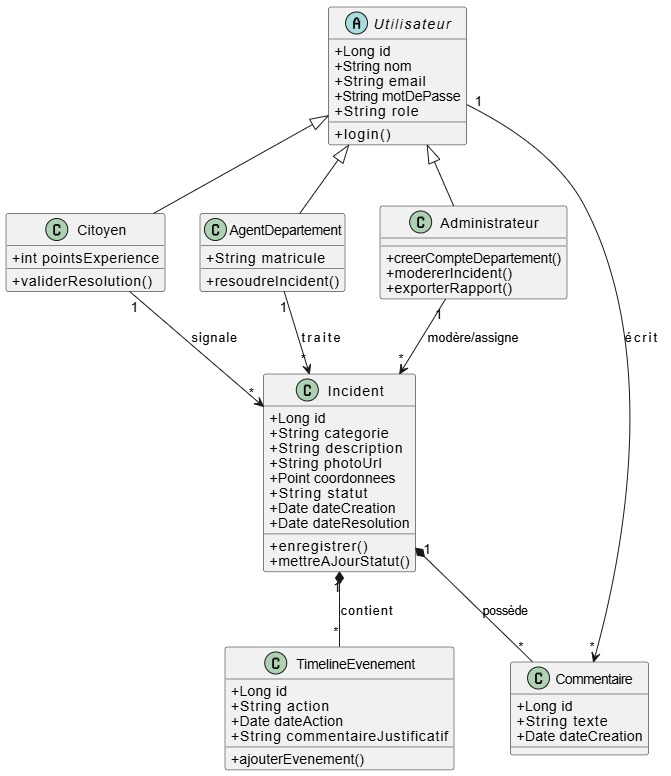
\includegraphics[width=0.9\textwidth]{classes_sprint4.jpg}
    \caption{Diagramme de classes du Sprint 4}
    \label{fig:class_sprint4}
\end{figure}

% ------------------------------------------------------------------------------
% 6. RÉALISATION
% ------------------------------------------------------------------------------
\section{Réalisation}

\subsection{Modélisation de la Timeline en Base de Données}
Chaque incident possède un historique d'états géré par la table \texttt{table_incident_timeline} :
*   \texttt{id} (BIGINT, PK)
*   \texttt{incident_id} (FK vers la table incident)
*   \texttt{status} (VARCHAR, ex : SOUMIS, AFFECTE, A_VALIDER_FIX, RESOLVED)
*   \texttt{comment} (TEXT, stocke le motif du rejet de l'Admin ou les notes d'affectation)
*   \texttt{actor_name} (VARCHAR, nom de l'acteur ayant déclenché l'événement)
*   \texttt{created_at} (TIMESTAMP)

\subsection{Implémentation de la Modération et des Commentaires}
La couche service Spring Boot implémente la modération finale de la preuve de fixation :
\begin{verbatim}
@Service
public class ModerationService {
    @Autowired
    private IncidentRepository incidentRepository;
    @Autowired
    private TimelineRepository timelineRepository;
    @Autowired
    private UserProfileRepository userRepository;

    @Transactional
    public void moderateFixation(Long incidentId, boolean isAccepted, String reason, String adminName) {
        Incident incident = incidentRepository.findById(incidentId)
            .orElseThrow(() -> new ResourceNotFoundException("Incident non trouvé"));

        IncidentTimeline log = new IncidentTimeline();
        log.setIncident(incident);
        log.setActorName(adminName);
        log.setCreatedAt(LocalDateTime.now());

        if (isAccepted) {
            incident.setStatus("RESOLVED");
            log.setStatus("RESOLVED");
            log.setComment("Réparation validée par l'administration.");
            
            // Créditer les points au citoyen
            UserProfile citizen = incident.getUser();
            citizen.setImpactPoints(citizen.getImpactPoints() + incident.getCategory().getBasePoints());
            userRepository.save(citizen);
        } else {
            // Rejeter la fixation et remettre en cours pour nouvelle intervention
            incident.setStatus("EN_COURS");
            log.setStatus("EN_COURS");
            log.setComment("Réparation rejetée. Motif : " + reason); // Motif de rejet obligatoire
        }
        
        incidentRepository.save(incident);
        timelineRepository.save(log);
    }
}
\end{verbatim}

\subsection{Enchaînement des interfaces réalisées}
Sur l'application mobile Flutter, le citoyen ouvre un incident. Il visualise son statut de résolution (fixé ou non) directement sur la carte interactive. Si l'incident est résolu (avec photo preuve validée), le citoyen peut alors taper un commentaire (ex : « Merci pour la réactivité, le trou est bien bouché ! ») ou attribuer une note sous forme d'étoiles pour évaluer la qualité du correctif, favorisant la transparence démocratique locale. L'accès à la timeline chronologique détaillée de l'incident et aux détails de modération reste réservé à la console d'administration.

\section*{Conclusion}
Le Sprint 4 clôture le cycle de vie de la plateforme \textit{SafeCity-Connect} en intégrant un workflow de modération rigoureux des réparations et un espace de commentaires interactif. L'enchaînement des interfaces Flutter et Angular garantit un flux d'information transparent et continu : du signalement citoyen géo-localisé à la fixation par photo preuve, validée par l'administration et commentée par la communauté.

\newpage

% Conclusion générale
% ==============================================================================
% FICHIER : conclusion_generale.tex
% Description : Conclusion Générale
% Auteurs : Dhia Fersi & Mohamed Iyed Amiri (ISET Bizerte)
% Organisme d'accueil : HRMAPS
% ==============================================================================

\chapter*{Conclusion Générale}
\addcontentsline{toc}{chapter}{Conclusion Générale}

Le travail présenté dans ce rapport s'inscrit dans le cadre du développement de la plateforme citoyenne intelligente \textbf{SafeCity-Connect}, réalisée sous la tutelle de notre organisme d'accueil \textbf{HRMAPS}. Ce projet de fin d'études a représenté pour nous un défi technologique et méthodologique captivant, visant à moderniser la gestion des infrastructures urbaines par l'implication active des citoyens et l'apport de l'intelligence artificielle.

Tout au long de ce projet, nous avons suivi une démarche structurée :

En premier lieu, la phase de cadrage et d'étude de l'existant a permis de cerner la problématique complexe de la réactivité municipale et du désengagement des citadins face à la dégradation de leur espace public. C'est sur ces constatations que s'est fondée notre proposition d'une plateforme connectée bidirectionnelle.

En second lieu, l'analyse détaillée des besoins a permis de dégager précisément les profils des utilisateurs (Citoyens, Administrateurs communaux) et de délimiter l'ensemble des cas d'utilisation UML associés. Nous avons identifié la sécurité (via Keycloak SSO), le traitement IA (YOLO) et l'ergonomie responsive comme des exigences non fonctionnelles de premier ordre.

En troisième lieu, lors de la phase de conception, nous avons conçu une architecture moderne, distribuée et hautement sécurisée en nous basant sur le protocole OAuth2 et le flux PKCE. De plus, nous avons élaboré le modèle de données géospatial PostGIS nécessaire pour stocker nativement les géométries et optimiser les calculs géographiques complexes.

En quatrième lieu, la phase de réalisation a concrétisé cette étude à travers l'assemblage de notre Tech Stack : Spring Boot 3.2 pour le cœur d'API, Angular 18 pour la console d'administration web, Flutter pour l'application mobile citoyen et technique, Keycloak pour la gestion de sécurité unifiée, et le module YOLO AI. L'orchestration par Docker Compose a permis d'assurer l'homogénéité et la portabilité des services développés.

Ce projet a pleinement atteint les objectifs initiaux fixés. Les citoyens disposent d'une application mobile Flutter ergonomique pour signaler en temps réel les incidents, commenter les réparations et suivre la timeline, tout en étant encouragés par les points d'impact. De leur côté, les gestionnaires profitent d'un outil de pilotage cartographique (Heatmap PostGIS) et documentaire (exports PDF/Excel) performant.

\section*{Perspectives d'avenir}
Bien que la plateforme soit pleinement opérationnelle, plusieurs axes d'évolution prometteurs peuvent être envisagés pour enrichir \textit{SafeCity-Connect} à l'avenir :

\begin{itemize}
    \item \textbf{Intégration d'un modèle d'IA de production} : Remplacer la simulation d'IA actuelle par un réseau de neurones YOLOv8/v9 entraîné spécifiquement sur des jeux de données réels de dégradations urbaines.
    \item \textbf{Notifications Push via Firebase (FCM)} : Intégrer Firebase Cloud Messaging pour envoyer des notifications push instantanées sur l'application Flutter des citoyens à chaque étape de la timeline (ex : acceptation ou rejet motivé du correctif par l'Admin).
    \item \textbf{Mode Hors-Ligne (Offline Sync)} : Permettre aux citoyens et aux agents techniques de capturer des incidents et photos de fixation sans connexion internet, les données étant stockées localement (SQLite/Hive) et synchronisées automatiquement dès le retour du réseau.
    \item \textbf{Module d'optimisation de tournées} : Intégrer un algorithme d'optimisation de trajet (type pgRouting) pour tracer sur l'application mobile des agents l'itinéraire optimal de résolution des incidents affectés.
\end{itemize}

En définitive, ce Projet de Fin d'Études a constitué une opportunité exceptionnelle de mettre en pratique nos connaissances académiques acquises au sein de l'ISET Bizerte, tout en nous familiarisant avec les exigences d'une entreprise innovante comme HRMAPS. Nous espérons que \textit{SafeCity-Connect} posera les premiers jalons de la transition numérique vers des villes plus intelligentes, réactives, vertes et à l'écoute constante de leurs habitants.

\newpage

% Bibliographie / Webographie
% ==============================================================================
% FICHIER : bibliographie.tex
% Description : Bibliographie et Webographie
% Auteurs : Dhia Fersi & Mohamed Iyed Amiri (ISET Bizerte)
% Organisme d'accueil : HRMAPS
% ==============================================================================

\thispagestyle{plain}
\chapter*{Bibliographie et Webographie}
\addcontentsline{toc}{chapter}{Bibliographie et Webographie}

% --- BIBLIOGRAPHIE ---
\section*{Références Bibliographiques}
\begin{enumerate}
    \item \textbf{C. Albin} (2020). \textit{Conception d'applications web modernes avec Spring Boot et Angular}. Éditions Eyrolles, 2ème édition.
    \item \textbf{J. Redmon, S. Divvala, R. Girshick, and A. Farhadi} (2016). \textit{You Only Look Once: Unified, Real-Time Object Detection}. CVPR 2016, pp. 779-788.
    \item \textbf{R. S. Pressman} (2015). \textit{Génie logiciel: Méthodes et Pratiques}. Éditions Pearson France, 8ème édition.
    \item \textbf{R. Obe and L. Hsu} (2021). \textit{PostGIS in Action}. Manning Publications, 3ème édition.
\end{enumerate}

\vspace{0.5cm}

% --- WEBOGRAPHIE ---
\section*{Références Webographiques}
\begin{enumerate}
    \item \textbf{Documentation Officielle de Spring Boot} \\
    \textit{Spring Boot Framework - Version 3.2.x} \\
    URL : \href{https://spring.io/projects/spring-boot}{https://spring.io/projects/spring-boot} \\
    Consulté le 15 février 2026.
    
    \item \textbf{Documentation Officielle d'Angular} \\
    \textit{Angular Developer Guide - Version 18.x} \\
    URL : \href{https://angular.dev}{https://angular.dev} \\
    Consulté le 20 février 2026.
    
    \item \textbf{Documentation Officielle de Keycloak} \\
    \textit{Keycloak - Open Source Identity and Access Management for Modern Applications} \\
    URL : \href{https://www.keycloak.org/documentation}{https://www.keycloak.org/documentation} \\
    Consulté le 10 mars 2026.
    
    \item \textbf{Documentation Officielle de PostGIS} \\
    \textit{PostGIS Spatial Database Extender for PostgreSQL} \\
    URL : \href{https://postgis.net/documentation/}{https://postgis.net/documentation/} \\
    Consulté le 18 mars 2026.
    
    \item \textbf{Site Officiel de HRMAPS} \\
    \textit{HRMAPS -- Éditeur de logiciels de gestion des talents et SIRH} \\
    URL : \href{https://www.hrmaps.fr}{https://www.hrmaps.fr} \\
    Consulté le 05 avril 2026.
    
    \item \textbf{Documentation Leaflet.js} \\
    \textit{Leaflet - an open-source JavaScript library for mobile-friendly interactive maps} \\
    URL : \href{https://leafletjs.com/}{https://leafletjs.com/} \\
    Consulté le 12 avril 2026.
    
    \item \textbf{Repository YOLOv8 d'Ultralytics} \\
    \textit{Ultralytics YOLO -- Real-time Object Detection and Image Segmentation} \\
    URL : \href{https://github.com/ultralytics/ultralytics}{https://github.com/ultralytics/ultralytics} \\
    Consulté le 25 avril 2026.
\end{enumerate}


\end{document}
